\documentclass[a4paper,11pt,titlepage,abstract,numbers=noenddot,automark,mnsy,intlimits,rgb,dvipsnames]{report}
\usepackage[hidelinks, colorlinks=true, urlcolor=blue, linkcolor=black, citecolor=blue]{hyperref}
\usepackage[english]{babel}
\usepackage{unicode-math}
\usepackage{xunicode}
\usepackage{url}
\usepackage{cite}
\usepackage{graphicx}
\usepackage[justification=centering, labelfont=bf]{caption}
\usepackage{float}
\usepackage{pgfgantt}
\usepackage{marvosym}
\usepackage{siunitx}
\usepackage{multirow}
\usepackage[nottoc]{tocbibind}
\usepackage{indentfirst}
\usepackage{afterpage}
\usepackage{minted}
\usepackage{tabularx}
\usepackage{tikz}
\usepackage[toc,page]{appendix}
\usepackage{svg}
\usepackage[chapter]{algorithm}
\usepackage{algorithmic}
\usetikzlibrary{arrows,positioning}
\usepackage{fontspec}
\usepackage{parskip}
\usepackage{fancyhdr}
\usepackage{titlesec}

\defaultfontfeatures{Scale=MatchLowercase}
\setmainfont[Ligatures=TeX,
BoldFont=texgyrepagella-bold.otf,
BoldItalicFont=texgyrepagella-bolditalic.otf,
ItalicFont=texgyrepagella-italic.otf]{texgyrepagella-regular.otf}
\setsansfont[Ligatures=TeX,
BoldFont=lmsans10-bold.otf,
BoldItalicFont=lmsans10-boldoblique.otf,
ItalicFont=lmsans10-oblique.otf]{lmsans10-regular.otf}
\setmonofont[BoldFont=lmmonolt10-bold.otf,
BoldItalicFont=lmmonolt10-boldoblique.otf,
ItalicFont=lmmono10-italic.otf,
SlantedFont=lmmonoslant10-regular.otf]{lmmono10-regular.otf}
\setmathfont{texgyrepagella-math.otf}
\setmathfont[range={\mathcal,\mathbfcal},StylisticSet=1]{xits-math.otf}
\setlength{\parindent}{24pt}
\setcounter{secnumdepth}{5}
\setcounter{tocdepth}{1}


 
\pagestyle{fancy}
\fancyhf{}
\fancyhead[LE,RO]{Héctor Ramón}
\fancyhead[RE,LO]{\leftmark}
\fancyfoot[RE]{Final degree project}
\fancyfoot[LO]{\emph{Web platform for multiplayer programming games}}
\fancyfoot[LE,RO]{\thepage}

\renewcommand{\footrulewidth}{0.5pt}
\setlength{\marginparwidth}{0pt}
\setlength{\parskip}{0.8em}


\titleformat{\chapter}{\normalfont\bfseries}{\Huge\thechapter}{20pt}{\Huge}
\newcommand*{\fullref}[1]{\hyperref[{#1}]{\autoref*{#1} \nameref*{#1}}}

\begin{document}
\begin{titlepage}
\begin{center}
\textsc{\Large Degree Final Project}
\\[1.5cm]
\rule{\linewidth}{0.5mm}
\\[0.4cm]
{\huge
\bfseries
Platform for massive multiplayer programming games
\\[0.4cm]
}
\rule{\linewidth}{0.5mm}
\\[0.3cm]
{\bfseries
Computation
}
\\[2.5cm]
\begin{center}
\large
Héctor Ramón Jiménez
\end{center}
{\small \emph{Advisor}}\\Jordi Petit Silvestre
\vfill
{\large
Facultat d'Informàtica de Barcelona\\\small Universitat Politècnica de Catalunya
}
\\[0.5cm]
{\large
\today
}
\end{center}
\end{titlepage}
\clearpage
\begin{abstract}
This project states that a platform for multiplayer programming games with a high
  number of players and long matches is needed. It provides a design of an open-source solution to satisfy this necessity
  and describes its implementation using a methodology based on continuous integration. Finally, the implemented solution
  is evaluated, concluding that it is a good candidate for such a platform.
\end{abstract}
\clearpage
\tableofcontents
\clearpage
\chapter{Introduction}
This chapter reviews the history of programming games, states the
personal motivation of the author, and details the structure of this report.
\section{Brief history of programming games}
\subsection{Playing games while programming}
In 1961, Victor Vyssotsky, a mathematician and computer scientist working at Bell Labs, along with Robert Morris Sr. and 
Doug McIlroy, created Darwin \cite{darwin}: the \textbf{first programming game}. This game was not played by a player with a controller.
Instead, Darwin could only be played by writing a computer program.

A \emph{programming game} is a computer game where the player does not directly interact with the game. Instead, the
player writes a computer program that plays the game. These computer programs are usually called artifficial
intelligences (\texttt{AIs}) because they try to make intelligent decisions to win the game.

Darwin consisted of two or more small programs, written by the players, that were loaded in memory. The main goal
of the game was to spread copies of your own program and find and kill the copies of other players. The game was only
played for a few weeks before Morris developed an ultimate program, as no-one managed to produce anything that could
defeat it.

Since then, many other programming games have been created \cite{pg}. Some of them are even commercial games, like
SpaceChem \cite{spacechem}.
\subsection{Playing with other people}
With the arrival of the Internet and the World Wide Web, there was nothing stopping people from
developing web platforms for multiplayer programming games.

A \emph{multiplayer programming game} is a programming game where multiple players compete with each other to win the
game. Thus, the game becomes a challenge where strategy and programming skills make the difference.

These web platforms allow players to compete with each other easily. For example, Robot Game
\cite{robotgame} is a website where anyone can upload an \texttt{AI} written in \texttt{}Python\texttt{} and compete with other people.
\subsection{Playing while learning}
Writing \texttt{AIs} can be a really fun and rewarding experience because the game allows the players to see how their
algorithms work visually, while competition motivates them to learn and improve.

It comes as no surprise, then, that programming games are being used in schools, as gamification \cite{gamification},
to teach students different programming techniques.
For instance, an \texttt{AI} programming challenge is held every semester in the Barcelona School of
Informatics (FIB) where students enrolled in the subject Data Structures and Algorithms (EDA) \cite{eda}
compete with each other in a multiplayer programming game using the Jutge.org platform \cite{jutge}.
\section{Personal motivation}
I love videogames. Ever since my father introduced me to my first computer when I was 3 years old.
I was immediately hooked. I started playing simple puzzle games, while discovering first person shooters and strategic
games soon after.

Videogames were the main reason I chose to study computer science. I learned my first
programming language because I wanted to open a website
to share my passion about videogames. I was 10 years old back then. Programming is a really important
facet of my life.

Studying computer science has made me love videogames even more. When I a see videogame now, I can try to
imagine the logic
behind it. I can try to picture the different algorithms involved. I imagine thousands of bits correctly aligned,
flowing and changing constantly, while they follow some complex logic. For me, the fact that a videogame is
able to show how its code works visually is truly fascinating.

Programming games mix two of my passions: videogames and programming. So when this project was offered to me,
I thought it was the \textbf{perfect fit}.
\section{Report structure}
This report consists of four different parts. Each one of them describes a vital phase in the development of
the project:
\begin{description}
\item[Formulation]
Identifies and analyzes the problem to solve, it specifies the scope of
  the project, and it shows the design of the solution.
\item[Planning]
Details the time plan and the budget to develop the project.
\item[Implementation]
Describes the development of the different components that compose the solution.
\item[Evaluation]
Describes the validation methodology, it reviews the time management and economic cost,
  and it discusses the sustainability and legality issues of the project.
\end{description}
\part{Formulation}
\chapter{Analysis}
This chapter details the problem that this project aims to solve and it decides whether there is some existing
solution that may apply to solve this problem.
\section{The requirement}
\label{requirement}
The advisor of this project is one of the founders of the Jutge.org platform. Also, he is deeply involved in the \texttt{AI}
programming challenge organized in the \texttt{EDA} subject in the FIB.

Currently, the contest strategy is based on a round system. All the students play at least one match per round. Players
that lose a match play against other losers. At the end, the player that loses the last match is eliminated from the contest.

Clearly, this strategy has one main drawback: eliminated students stop playing. Hence, their learning process halts completely.
This could be solved using a simple score system, but it would still be patching the main issue: the
programming games used do not support a huge amount of players natively.

The aim of this project is to provide an easy way to develop multiplayer programming games featuring huge worlds,
long matches and a massive amount of players in real-time. This will make players feel attached to the match,
programs will need to adapt constantly as they play with everyone at the same time. As a consequence, this project will
finally allow to improve the strategy used in the \texttt{EDA} progamming challenge.
\section{State of the art}
\label{state_of_the_art}
There are many platforms that offer \texttt{AI} programming challenges. Some examples are:
\begin{description}
\item[Google's \texttt{AI} programming challenge \cite{google_ai}]
The university of Waterloo organized some \texttt{AI} programming challenges
  sponsored by Google during 2010-2011.
\item[Battlecode \cite{battlecode}]
A website that organizes an \texttt{AI} programming challenge every year where anyone can
  compete alone or in a team.
\item[CodinGame \cite{codingame}]
A website that has many \texttt{AI} programming contests, which can help players to apply for
  specific jobs.
\item[\texttt{EDA} competition \cite{eda}]
An \texttt{AI} programming challenge is held every semester in the Barcelona School of
  Informatics (FIB) where students compete with each other using the Jutge.org platform \cite{jutge}.
\end{description}
However, all of these platforms feature multiplayer programming games with short matches played by a
small number of players. As a consequence, multiple matches with different players are necessary to decide who wrote
the best \texttt{AI}.

Given that there is no pre-made solution that fits the project's requirement, a new brand solution is necessary.
\section{Stakeholders}
Given the requirement described in \autoref{requirement}, the different users that will use the platform are considered:
\begin{description}
\item[Game programmers]
They want to create \texttt{MMPGs} easily. They want to focus on programming the game logic and the
  game viewer, without worrying about internal aspects of the platform.
\item[Players]
They will develop \texttt{}AI\texttt{}s for a concrete game and upload them to the web platform at any time during
  the game match.
\item[Viewers]
They want to watch the match unfold in real-time.
\item[Administrators]
They want to control the game. They want to supervise, start, stop or pause the game, and obtain
  the final scores of every player.
\end{description}
\clearpage
\chapter{Objectives}
\label{specification}
This chapter details the different objectives that the project must fullfill in order to satisfy the requirement stated in
the previous chapter.
\section{Main objective}
Develop a set of components that ease the creation and the usage of massive multiplayer programming games.
\section{Secondary objectives}
\label{secondary_objectives}
\begin{description}
\item[Develop an abstract game engine]
Any experienced programmer must be able to create new games for the platform.
\item[Allow hot-swapping of \texttt{AIs}]
Players must be able to change the code of their current \texttt{AIs} in the middle of a match.
\item[Implement a real-time webviewer]
Players must be able to watch in real-time how the game unfolds in a web browser.
\item[Create a control panel]
Administrators must be able to play, pause and stop the game and also see a ranking of the current match.
\item[Make the infrastructure scalable and stable]
The underlying infrastructure must be able to handle huge worlds and a large number of \texttt{}AI\texttt{}s without
  hindering performance. Moreover, the platform must be secure and fault-tolerant; \texttt{AIs} must not be able to cheat
  or affect the platform negatively.
\item[Create a game example]
A multiplayer programming game will be created to test and show that the platform works correctly.
\end{description}
\clearpage
\chapter{Design}
\label{design}
The design of the platform has to allow game developers to implement \texttt{MMPGs} easily. Hence, it is necessary to keep
the number of components and dependencies at bay.
\begin{figure}[H]
\begin{center}
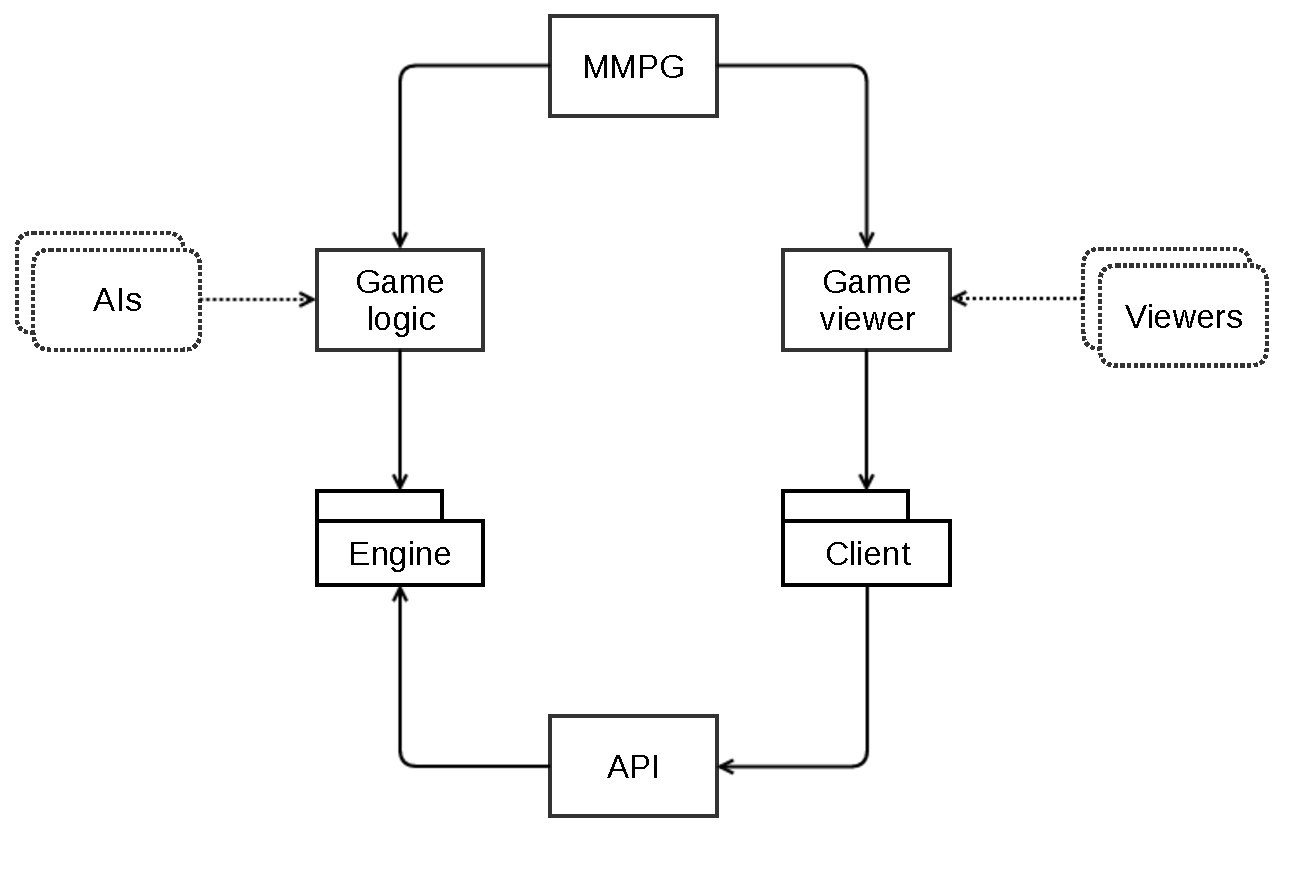
\includegraphics[scale=0.5]{graphs/mmpg_design.pdf}
\end{center}
\caption{The design of an \texttt{MMPG}}
\label{mmpg_graph}
\end{figure}
\autoref{mmpg_graph} shows a diagram of the different components that compose an \texttt{MMPG} and their dependencies. As it is shown,
game developers only need to implement two components to create an \texttt{MMPG}: the game logic and the game viewer. This is
quite logical, since these are the only two components that are game-specific.

Hence, a massive multiplayer programming game using the platform consists of:
\begin{description}
\item[Engine]
A library that implements basic features needed by any \texttt{MMPG}. The engine exposes a set
  of classes that must be extended to build the game logic.
\item[\texttt{API}]
A component that exposes \texttt{HTTP} endpoints that allow to interact with an underlying engine. It
  usually handles requests from a game viewer using the client library.
\item[Client]
A library that implements a set of useful classes to communicate with an \texttt{API} and implement
  game viewers.
\item[Game logic]
It includes the game world definition and the rules of the game and executes the different \texttt{AIs}.
  It is built on top of the engine.
\item[Game viewer]
It allows viewers to watch game matches. Also, it makes players able to upload new \texttt{AIs}. It uses
  the client library to connect to the \texttt{API}.
\end{description}
\clearpage
\chapter{License}
\section{Code}
The \texttt{MMPG} platform code and the game example will be released under The MIT License \cite{mit_license}.
\section{Documents}
This monitoring report and the final document related with the \texttt{MMPG} platform hosted in
\url{https://github.com/hecrj/mmpg} will be released under the
Creative Commons Attribution-NonCommercial-ShareAlike 4.0 International \cite{cc_license} license.
\clearpage
\part{Planning}
\chapter{Time plan}
\section{Estimated project duration}
The project starts the September 15th, 2015 and its deadline is the January 25th, 2016. Thus,
the project will take approximately 4 months to be completed.
\section{Tasks}
This section details the different tasks and subtasks that need to be completed in order
to finish the project successfully. Every task is provided with a description, an expected duration,
possible complications and task dependencies.
\subsection{Project management course}
The project management course aims to help lead the project in the right direction. In this task,
different parts of the project are defined: context and scope, temporal planning, and
economic viability.
\begin{description}
\item[Expected duration]
75 hours.
\item[Possible complications]
None. The course is entirely guided and feedback is
  regularly provided to ensure the author can finish it properly.
\item[Task dependencies]
None.
\end{description}
\subsection{Analysis and design}
In this task, the project requirements are analyzed and a solution is designed to satisfy them.
\begin{description}
\item[Expected duration]
10 hours.
\item[Possible complications]
Some minor details might change during the implementation. It is
  important to focus on the \emph{big picture} of the project.
\item[Task dependencies]
None.
\end{description}
\subsection{Engine}
A library that will allow game programmers to build games and wire them to the platform. The codebase will implement the features that are independent of the final game and, therefore, can be reused.
\begin{description}
\item[Expected duration]
70 hours
\item[Possible complications]
\texttt{AI} memory management might be difficult.
  The author may need to learn low-level instructions to control OS's processes.
\end{description}
\subsubsection{API}
A web-server that notifies its subscribers of the changes that occur in the game world.
\begin{description}
\item[Expected duration]
50 hours
\item[Possible complications]
The author needs to learn \texttt{Go}, which might take some time.
\end{description}
\subsection{Client}
A library that handles a connection with the \texttt{API}. Game programmers will be able to use it to build
the real-time webviewers of their games. It will be programmed in \texttt{}Javascript\texttt{}, using \texttt{Coffeescript}.
\begin{description}
\item[Expected duration]
30 hours
\item[Possible complications]
The author needs to learn \texttt{Coffeescript}, which might take some time.
\end{description}
\subsection{Control panel}
Allows administrators to supervise the games, start, stop and pause current matches, and obtain the
scores of every player.
\begin{description}
\item[Expected duration]
35 hours
\item[Possible complications]
None.
\end{description}
\subsection{Game example}
A massive multiplayer programming game will be developed to test that the underlying
engine and infrastructure work as intended. This task will be splitted in other two: logic and viewer.
\subsubsection{Logic}
During this task, the main logic of the game will be developed on top of the engine.
This includes the different game rules and the game world.
\begin{description}
\item[Expected duration]
50 hours
\item[Possible complications]
Balancing the game could be really hard.
\item[Task dependencies]
Engine.
\end{description}
\subsubsection{Viewer}
In this task, a web-viewer that shows the game world in real-time will be developed using the \texttt{API}.
\begin{description}
\item[Expected duration]
50 hours
\item[Possible complications]
Loading a huge game world might be complicated.
\item[Task dependencies]
\texttt{API}.
\end{description}
\subsection{Testing and polishing}
In this task, the platform will be tested under heavy load to ensure its stability and scalability.
\begin{description}
\item[Expected duration]
40 hours
\item[Possible complications]
Components might need to change if some unexpected bottleneck is detected.
\item[Task dependencies]
Game example.
\end{description}
\subsection{Project memory}
During this task, a document explaining how the project was developed will be written.
\begin{description}
\item[Expected duration]
40 hours
\item[Possible complications]
None.
\item[Task dependencies]
Engine. It will be written in different parts, after each task is finished.
\end{description}
\subsection{Oral presentation}
Once the project memory is finished, the author will prepare the final oral presentation.
\begin{description}
\item[Expected duration]
10 hours
\item[Possible complications]
Live examples must be well-prepared beforehand.
\item[Task dependencies]
Project memory.
\end{description}
\clearpage
\section{Time table}
\autoref{planning_time_table} summarizes the duration of every task described in the previous section.
The total duration of the project is expected to be 460 hours. The author will need to work
$\frac{460 \: hour}{16 \: week} \simeq 29 \: hour/week$ to finish the project before the deadline, which seems reasonable.
\begin{figure}[H]
\begin{center}
\begin{tabular}{l S}
\textbf{Task} & \textbf{Expected duration (h)}\\
\hline
Project management course & 75\\
\hline
Analysis and design & 10\\
\hline
Engine & \\
\hspace{1em}
Learning & 5\\
\hspace{1em}
Implementation & 50\\
\hspace{1em}
Testing & 14\\
\hspace{1em}
Integration & 1\\
\hline
Client & \\
\hspace{1em}
Learning & 10\\
\hspace{1em}
Implementation & 25\\
\hspace{1em}
Testing & 10\\
\hspace{1em}
Integration & 5\\
\hline
API & \\
\hspace{1em}
Learning & 5\\
\hspace{1em}
Implementation & 20\\
\hspace{1em}
Testing & 3\\
\hspace{1em}
Integration & 2\\
\hline
Control panel & \\
\hspace{1em}
Learning & 5\\
\hspace{1em}
Implementation & 20\\
\hspace{1em}
Testing & 5\\
\hspace{1em}
Integration & 5\\
\hline
Game example & \\
\hspace{1em}
Logic & 50\\
\hspace{1em}
Viewer & 50\\
\hline
Testing and polishing & 40\\
\hline
Project memory & 40\\
\hline
Oral presentation & 10\\
\hline
\hline
\textbf{Total} & 460\\
\end{tabular}
\end{center}
\caption{Planning time table}
\label{planning_time_table}
\end{figure}
\section{Timeline}
\autoref{planning_timeline} shows the expected timeline of the project, taking into consideration
task dependencies.
\begin{figure}[H]
\noindent\resizebox{\textwidth}{!}{
\begin{ganttchart}[hgrid, vgrid]{1}{25}
\gantttitle{2015}{20}
\gantttitle{2016}{5}
\\
\gantttitle{September}{5}
\gantttitle{October}{5}
\gantttitle{November}{5}
\gantttitle{December}{5}
\gantttitle{January}{5}
\\
\ganttbar{Project management}{3}{8}
\\
\ganttbar{Analysis and design}{4}{5}
\\
\ganttbar{Engine}{6}{10}
\\
\ganttbar{Client}{11}{13}
\\
\ganttbar{API}{14}{15}
\\
\ganttbar{Control panel}{16}{17}
\\
\ganttbar{Game example - logic}{11}{18}
\\
\ganttbar{Game example - viewer}{16}{20}
\\
\ganttbar{Testing and polishing}{21}{22}
\\
\ganttbar{Project memory}{11}{23}
\\
\ganttbar{Oral presentation}{24}{24}
\ganttlink{elem1}{elem2}
\ganttlink{elem2}{elem3}
\ganttlink{elem3}{elem4}
\ganttlink{elem4}{elem5}
\ganttlink{elem2}{elem6}
\ganttlink{elem4}{elem7}
\ganttlink{elem6}{elem8}
\ganttlink{elem7}{elem8}
\ganttlink{elem2}{elem9}
\ganttlink{elem9}{elem10}
\end{ganttchart}
}
\caption{Planning timeline}
\label{planning_timeline}
\end{figure}
\chapter{Budget}
\label{budget}
\section{Hardware resources}
The project will be developed using a personal desktop computer and a laptop. Also, a monitor,
a keyboard and a mouse are needed to use the desktop computer. There is no other hardware needed.
\begin{table}[H]
\centering
\begin{tabular}{l S S S}
\textbf{Hardware} & \textbf{Cost (\EURtm)} & \textbf{Useful life (years)} & \textbf{Amortized cost (\EURtm)}\\
\hline
Desktop computer & 2600.00 & 4 & 34.13\\
Personal laptop & 1000.00 & 4 & 13.13\\
Monitor Acer XB270HU & 750.00 & 4 & 9.85\\
Mouse Corsair M60 & 60.00 & 4 & 0.79\\
Keyboard Corsair K70 RGB & 170.00 & 4 & 2.23\\
\hline
\hline
\multicolumn{3}{l }{\textbf{Total}}
 & 60.13
\end{tabular}
\caption{Hardware budget}
\label{Hardware budget}
\end{table}
\section{Software resources}

The software to develop the project is: Ubuntu, Sublime Text, a web-browser, \texttt{CLion}, \LaTeX{}, \texttt{Makefile}, \texttt{git}, \texttt{evince},
    \href{https://github.com/hecrj/hal/raw/master/doc/full/report.pdf}{\texttt{HAL}}, \texttt{}C\texttt{++}, \texttt{Go},
    \texttt{}Javascript\texttt{}, \texttt{Coffeescript}, and \texttt{WebGL}.

However, all that software can be used for free. \autoref{Software licenses} shows the licenses of most of the software needed.

Mozilla Firefox includes a \texttt{}Javascript\texttt{} engine and \texttt{evince} is included in Ubuntu.
Also, the \texttt{HAL} programming language is owned by the author of the project. \texttt{Jetbrains} allows students to use
\texttt{CLion} for free\footnote{\url{https://www.jetbrains.com/student/}} and
\texttt{Sublime Text} can be used without registration with no limitations\footnote{\url{http://www.sublimetext.com/2}}.
Therefore, there are no software costs.
\begin{table}[H]
\centering
\begin{tabular}{l l}
\textbf{Software} & \textbf{License}\\
\hline
Ubuntu & \url{http://www.ubuntu.com/about/about-ubuntu/our-philosophy}\\
\LaTeX{} & \url{https://latex-project.org/lppl/}\\
\texttt{git} & \url{https://git-scm.com/about/free-and-open-source}\\
\texttt{}C\texttt{++} & \url{https://gcc.gnu.org/onlinedocs/libstdc++/manual/license.html}\\
\texttt{Go} & \url{https://golang.org/project/}\\
Mozilla Firefox & \url{https://www.mozilla.org/en-US/foundation/licensing/}\\
\texttt{Coffeescript} & \url{https://github.com/jashkenas/coffeescript/blob/master/LICENSE}\\
\texttt{WebGL} & \url{https://www.khronos.org/legal/license/}\\
\end{tabular}
\caption{Software licenses}
\label{Software licenses}
\end{table}
\section{Human resources}
\autoref{Salary per role} the expected salary per project role. \autoref{Human resources budget} shows the
expected cost of the human resources according to project roles and their respective tasks.
\begin{table}[H]
\centering
\begin{tabular}{l S}
\textbf{Role} & \textbf{Payment (\EURtm / h)}\\
\hline
Project manager & 35.00\\
Software engineer & 40.00\\
Software developer & 30.00\\
\end{tabular}
\caption{Salary per role}
\label{Salary per role}
\end{table}
\begin{table}[H]
\centering
\begin{tabular}{l l S S}
\textbf{Role} & \textbf{Task} & \textbf{Time (h)} & \textbf{Cost (\EURtm)}\\
\hline
\multirow{3}{*}{Project manager}
 & Project management course & 75 & 2625.00\\
 & Project memory & 40 & 1400.00\\
 & Oral presentation & 10 & 350.00\\
\hline
\multirow{1}{*}{Software engineer}
 & Analysis and design & 10 & 400.00\\
\hline
\multirow{6}{*}{Software developer}
 & Engine & 70 & 2100.00\\
 & API & 50 & 1500.00\\
 & Client & 30 & 900.00\\
 & Control panel & 35 & 1050.00\\
 & Game example & 100 & 3000.00\\
 & Testing and polishing & 40 & 1200.00\\
\hline
\hline
\multicolumn{2}{l }{\textbf{Total}}
 & 460.00 & 14525.00
\end{tabular}
\caption{Human resources budget}
\label{Human resources budget}
\end{table}
\section{Other resources}
\subsection{Electricity}
Electricity will be needed to power the hardware. \autoref{Electricity budget} shows the power consumption,
the estimated time of usage, and the cost for every piece of hardware that needs an external source of power,
assuming 0.147358 \EURtm / kWh in Spain.
\begin{table}[H]
\centering
\begin{tabular}{l S S S}
\textbf{Hardware} & \textbf{Consumption (W)} & \textbf{Time of usage (h)} & \textbf{Cost (\EURtm)}\\
\hline
Desktop computer & 400 & 400 & 23.58\\
Laptop & 100 & 50 & 0.74\\
Monitor Acer XB270HU & 30 & 400 & 1.77\\
\hline
\hline
\multicolumn{3}{l }{\textbf{Total}}
 & 26.08
\end{tabular}
\caption{Electricity budget}
\label{Electricity budget}
\end{table}
\subsection{Internet connection}
An Internet connection will be necessary to perform all the tasks. The author will use its personal
internet connection most of the time, which costs 38\EURtm/month $\simeq$ 0.05\EURtm/h. It is expected to use the internet connection during the 30\% of the
total project's duration.
Thus, the estimated budget for the internet connection is
460h $\cdot$ 0.05\EURtm/h $\cdot$ 0.3 $=$ 7.28\EURtm.
\section{Total}
\autoref{Total budget} shows the total budget needed to develop the project. The 10\% of the total cost
is added to face any unforeseen contingencies.
\begin{table}[H]
\centering
\begin{tabular}{l S}
\textbf{Resource} & \textbf{Total cost (\EURtm)}\\
\hline
Hardware & 60.13\\
Software & 0.00\\
Human & 14525.00\\
Electricity & 26.08\\
Internet & 7.28\\
\hline
\hline
Subtotal & 14618.49\\
Contingency (10\%) & 1461.85\\
\hline
\multicolumn{1}{l }{\textbf{Total}}
 & 16080.34
\end{tabular}
\caption{Total budget}
\label{Total budget}
\end{table}
\part{Implementation}
\chapter{Methodology}
\label{methodology}
As seen in \autoref{design}, the platform to be implemented is composed of different components that communicate with
each other. Developing a single piece of software is a difficult task, but it becomes even harder when this piece of software
communicates with other software, especially when both are being developed at the same time; changes made in
the public interface of some component can break other components.

Therefore, components will break. Developers are humans, and humans make mistakes. Thus, in order to be productive,
it is necessary to detect when a component breaks as soon as possible. That way, components can be fixed before more changes
are made and fixing it becomes a nightmare.

In order to ensure that all the components of the platform keep working during the entire implementation process, and also
detect and fix issues as soon as possible, the project was developed using an iterative methodology based on
continuous integration \autoref{ci}. This methodology consisted in:
\begin{enumerate}
\item
Develop a simple prototype of the platform.
\item
Run the prototype in some external server.
\item
When a change is made to any component:
\begin{enumerate}
\item
Apply and integrate the change in the server.
\item
Test that the prototype keeps working as expected.
\end{enumerate}
\end{enumerate}
This methodology has a lot of benefits. Not only it allows to detect mistakes as soon as they are made, but it also provides
a fully working prototype of the platform that can be shown to anyone. Thus, the development progress can be shown
transparently. Stakeholders can try the software while it is being developed and give feedback. In this case,
the prototype was available to the advisor of the project to assess and follow any progress closely.
\chapter{The first prototype}
\label{first_prototype}
The first step of the implementation process was to build a simple prototype of the platform.

This first prototype must implement the most basic feature of the platform and it also has to lay the foundations for extending
it easily. Therefore, it was decided that the first prototype should feature the first working versions of:
\begin{enumerate}
\item
The engine, running one simple player and notifying its actions to any subscribers.
\item
The \texttt{API}, subscribed to the engine and notifying its actions to clients.
\item
The client library, subscribed to the \texttt{API} and drawing the player actions in a web-browser.
\end{enumerate}
It is important to note that the engine and the client are libraries that can be used to build
game logic and game viewers, respectively. They cannot be executed as a stand-alone component. However,
game-specific code was included temporarily in this first prototype, which avoided unnecessary complexity\footnote{i.e.
creating game logic and game viewer components}.

The entire code of the \texttt{MMPG} platform can be found under the \texttt{mmpg} GitHub organization: \url{https://github.com/mmpg}.
\section{The first API}
\subsection{Programming language}
There are many programming languages that allow to create HTTP APIs, like Pyhton, \texttt{Ruby}, \texttt{Elixir}... However,
the language chosen to implement the \texttt{API} was the \texttt{Go} programming language because it includes native
libraries to build concurrent \texttt{REST} APIs and it is simpler, faster and easier-to-deploy than the alternatives.
\subsection{The subscriber hub}
The \texttt{API} needs to keep track of the different clients subscribed to it, and it also needs to be able to send data
to them.

A subscriber hub was developed using the native concurrency of Go. Basically, the hub runs an infinite loop in the
background that smartly monitors the connected clients; sending data or closing connections accordingly.
\subsection{The events endpoint}
A simple HTTP endpoint was created: \texttt{/events}. This endpoint accepted WebSocket connections and delegated them to the
hub.

After that, the \texttt{API} was ready to send data to game viewers in real-time.
\section{The first client}
\subsection{Programming language}
The client code needs to be executed by web-browsers, as game viewers are web-based.
Thus, it has to be written in \texttt{Javascript}, as it is supported by web-browsers natively.
\subsection{API subscription}
A WebSocket was connected to the \texttt{/events} endpoint, printing any received data in the \texttt{Javascript} console.
\section{The first engine}
\subsection{Programming language}
The engine needs to be fast, as the game logic will be built on top of it, and it also needs to access
low-level operative system operations, so it can limit how player programs are executed.

The most well-known programming languages that satisfiy these requirements are \texttt{C} and \texttt{C}++. However, \texttt{C}  is lacking
the capacity to represent abstractions and interfaces easily. Hence, \texttt{C}++ is the perfect alternative to implement
the engine, as it is efficient, object-oriented and it has access to the \texttt{}C\texttt{ POSIX }API\texttt{}, which allows to talk
directly to \texttt{UNIX}-based operative systems.
\subsection{The architecture}
When designing the first architecture of the engine, it was important to take its requirements into account:
\begin{enumerate}
\item
The engine must not allow \texttt{AIs} to cheat.
\item
The engine must be scalable.
\item
\texttt{AIs} may be hot-swapped during a match.
\end{enumerate}
Thus, if the game logic and all the \texttt{AIs} were executed in the same process:
\begin{enumerate}
\item
\texttt{AIs} could access the memory related with the game logic or other \texttt{AIs}.
\item
\texttt{AIs} must be executed in the same machine.
\item
Updating an \texttt{AI} would require a rebuild of the entire game logic and other \texttt{AIs}, and a restart of the process.
\end{enumerate}
In other words, it would be really unsafe, inefficient and it would couple all the \texttt{AIs} and the game logic together.

Therefore, the architecture of the engine consisted of 3 types of processes:
\begin{description}
\item[Master process]
It represented the game-world server. The master process listened to requests coming from
  players and updated the game world accordingly. There was only one master process per runtime.
\item[Worker process]
It represented a pool of players. A worker process executed a set of players and
  managed them. There could be multiple workers per runtime.
\item[Player process]
It represented a player program. A player process read the game world from the
  master process and performed requests to change the game world.
\end{description}
Processes comunicated with each other using low-latency sockets. Thus, different workers could be executed
in different machines to achieve better performance.

\autoref{engine_arch} shows the hierarchy of an engine runtime with $N$ workers and $M = \sum_{i=0}^{N} M_i$ players.
\begin{figure}[H]
\begin{center}
\noindent\resizebox{\textwidth}{!}{
\begin{tikzpicture}[->,>=stealth',shorten >=1pt,auto,node distance=0.8cm,
    main node/.style={thick,circle,draw,minimum width=2.5cm}]

    \node[main node] (1) {master};

	\node[auto=false] (2) [below=of 1]{\ldots};
    \node[auto=false] (21) [left=of 2]{};
    \node[auto=false] (23) [left=of 21]{};
    \node[auto=false] (22) [right=of 2]{};
    \node[auto=false] (24) [right=of 22]{};

    \node[main node] (3) [left=of 23]{worker$_1$};
    \node[main node] (4) [right=of 24]{worker$_N$};

    \node[auto=false] (5) [below=of 3]{\ldots};
    \node[main node] (6) [left=of 5]{player$_{1,1}$};
    \node[main node] (7) [right=of 5]{player$_{1,{M_1}}$};

    \node[auto=false] (8) [below=of 4]{\ldots};
    \node[main node] (9) [left=of 8]{player$_{N,1}$};
    \node[main node] (10) [right=of 8]{player$_{N,{M_N}}$};


    \path (1) edge (3);
    \path (1) edge (4);

    \path (3) edge (6);
    \path (3) edge (7);

    \path (4) edge (9);
    \path (4) edge (10);
\end{tikzpicture}

}
\end{center}
\caption{Hierarchy of engine processes}
\label{engine_arch}
\end{figure}
\subsection{Inter-process communication}
As it was explained previously, the engine featured a decoupled architecture. Different processes were
executed and communicated with each other using sockets. However, implementing inter-process communication from
scratch would have been a real challenge by itself, and it was not the subject of this project. This is where a
messaging technology came in.

The most well-known messaging technologies out there are: \texttt{RabbitMQ}, \texttt{ZeroMQ} and \texttt{ActiveMQ}.

\texttt{RabbitMQ} implements
a broker architecture, which means that messages are queued on a central node before being sent to its destination.
This architecture is totally unnecessary for the engine, as we want to decouple components, and it would also add
some latency.

\texttt{ActiveMQ} can be used with a peer-to-peer architecture but, when compared with \texttt{ZeroMQ}, it is a
high-level library. Thus, controlling the type of communication or socket behaviour is not easy with \texttt{ActiveMQ}.

On the other hand, \texttt{ZeroMQ} \cite{zeromq} is an embeddable networking library that implements
low-latency socket communication. It manages low-level communication, while providing a flexible and easy-to-use interface.
Also, \texttt{ZeroMQ} has bindings available for the most well-known programming languages.

Thus, \texttt{ZeroMQ} was the library chosen to implement all the inter-process communication.
\subsection{The first master process}
The first master process consisted of two basic components:
\begin{description}
\item[The notifier]
It sent any given message through a \texttt{ZeroMQ} socket.
\item[The server]
It listened requests made by player processes and notified them through the notifier.
\end{description}
This components allowed the master process to act as a game server, while notifying the actions of the players to any
subscribers.
\section{Putting it all together}
Once the initial engine was finished, a simple \texttt{AI} was developed to simulate a player moving
while following a square shape. This way, it would be clear if the prototype worked correctly or not, as the web-viewer would need
to show this movement.

Then, the \texttt{API} was connected to the engine notifier and the received messages were directly delegated to the \texttt{API} hub,
which in turn were sent to any open clients.

Finally, once the \texttt{Javascript} console started showing the received events, a simple scene using \texttt{Three.js} was created in the
client. This scene featured a cube representing the player, whose position was updated with every received event.
\autoref{cube_movement} shows the observed result. The prototype was finished.
\begin{figure}[H]
\begin{center}
\noindent\resizebox{!}{15em}{
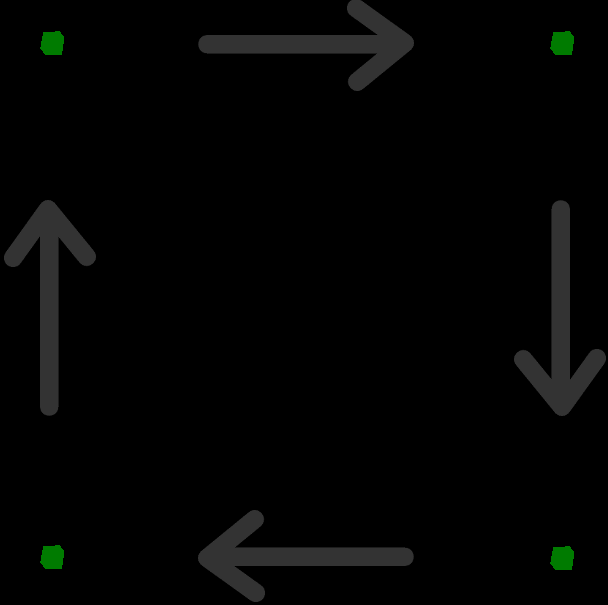
\includegraphics{images/cube_movement.png}
}
\end{center}
\caption{A cube that was moved by the player program}
\label{cube_movement}
\end{figure}
\section{Summary}
In this chapter, it is been described how the first prototype of the platform was built. A prototype that implemented the
most basic features of every component:
\begin{enumerate}
\item
The engine compiled and run players, and notified their actions to subscribers.
\item
The \texttt{API} subscribed to the engine and delegated the received events to all the connected clients.
\item
The client was able to connect to the \texttt{API} and receive events from the engine.
\end{enumerate}
The foundations of the platform were ready.
\chapter{Continuous integration}
Once the first prototype was finished, it was time to set up the integration server, as described in
\autoref{methodology}.
\section{The dedicated server}
First things first, an integration server to run the prototype was needed.

Initially, a server was requested to the project advisor. However, the university policy did not allow professors
to give root access to students. Root access was necessary because many different services might need to be installed during the
development of the platform\footnote{\texttt{ZeroMQ}, for example}. Therefore, it was decided to use an external cloud-host provider.

There are many providers that present cloud-hosting solutions\footnote{AWS \cite{aws}, DigitalOcean \cite{digital_ocean}, etc.}.
At the end, Linode \cite{linode} was the provider chosen, as the project developer already had experience with it and
the cheapest solution\footnote{This cost was covered with the contingency budget.} was enough to run the integration server.

A Linode 1GB \cite{linode} running \texttt{Ubuntu} was booted up to execute an
instance of the platform.
\section{The integration service}
The next step consisted in setting up an integration service.

Integration services keep track of some code repositories and can be configured to build and test the code when a change 
happens. Additionally, most of them can be configured to deploy changes when a build succeeds.

As it happened with cloud-hosting providers, there are many different integration
services\footnote{TravisCI \cite{travisci}, CircleCI \cite{circleci}, etc.}. Fortunately, most of them
are free to use for open-source projects, like this one. At the end, Semaphore \cite{semaphoreci} was the chosen
integration service. This decision was based in the experience the project developer had with the service, as it
also happened with the cloud-hosting provider.
\section{The integration process}
Semaphore was configured to trigger a build when any component
changed. If a build succeeded, then Semaphore deployed the changes to the Linode, where the changes were applied.

Changes were applied in the Linode using bare \texttt{git} repositories and script hooks. Basically,
when some changes were pushed to the repository, a script was executed that built and restarted the component.
These scripts were located in the repository itself, so they could be updated easily with the same process.

\autoref{build_process} shows the build process of the engine, while \autoref{deployment_process} shows
its deployment process.
\begin{figure}[H]
\begin{center}
\noindent\resizebox{30em}{!}{
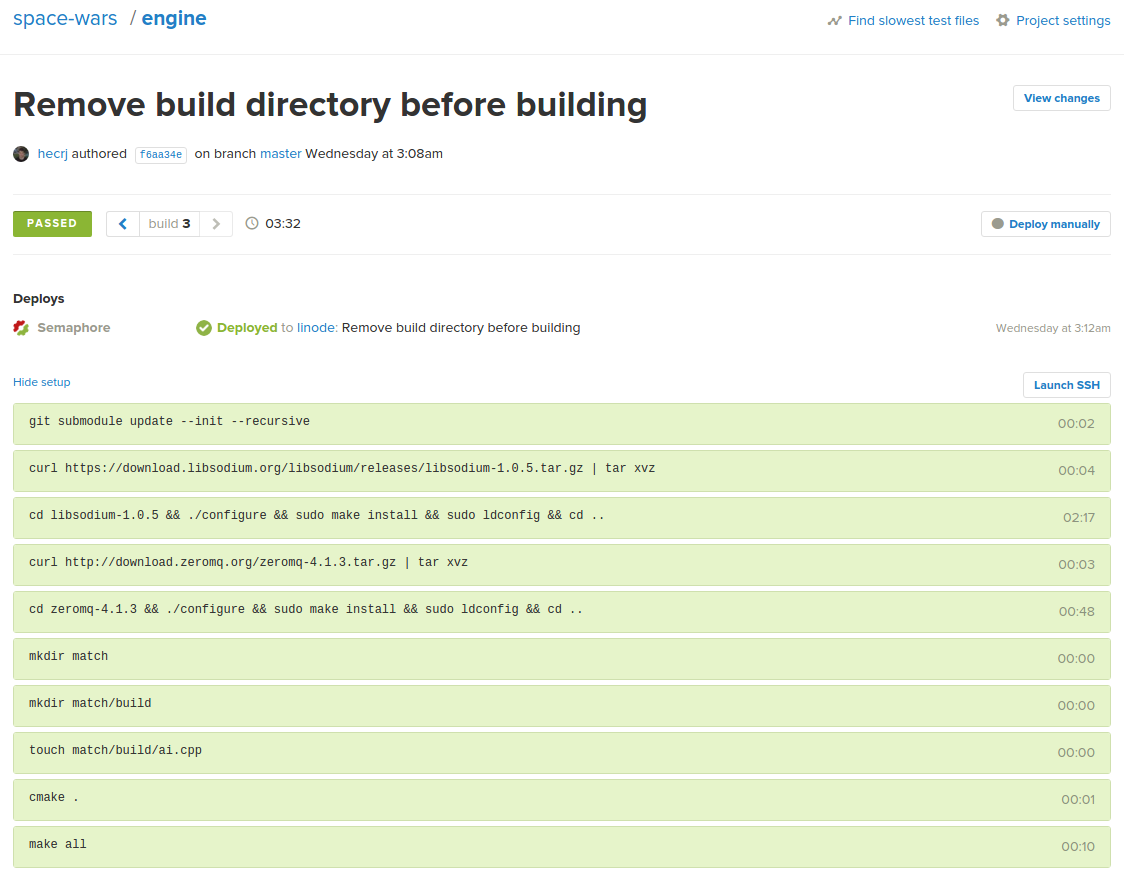
\includegraphics{images/build_process.png}
}
\end{center}
\caption{Semaphore build process}
\label{build_process}
\end{figure}
\begin{figure}[H]
\begin{center}
\noindent\resizebox{!}{30em}{
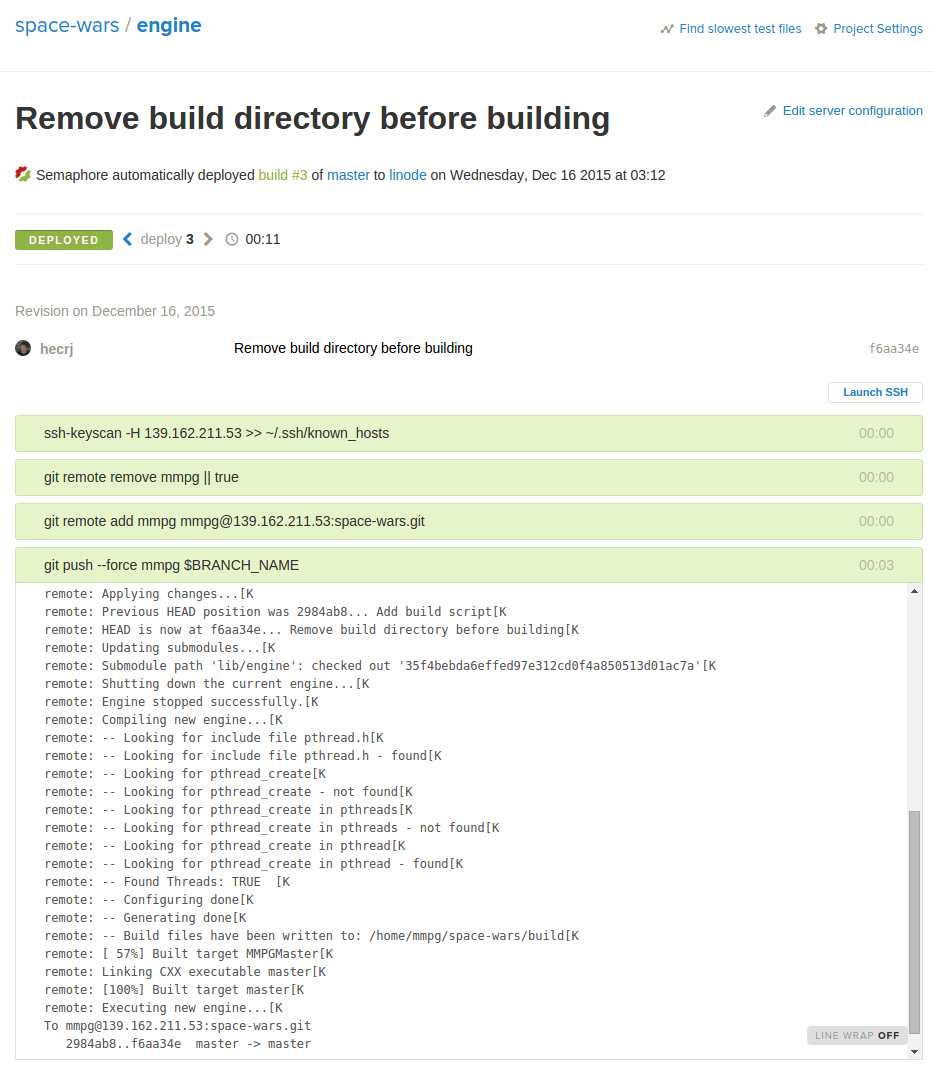
\includegraphics{images/deployment_process.png}
}
\end{center}
\caption{Semaphore deployment process}
\label{deployment_process}
\end{figure}
\chapter{The log system}
\label{log_system}
Matches of \texttt{MMPGs} are expected to last days or weeks, and while allowing viewers to watch the current state of
the match is mandatory, \texttt{AIs} will keep playing while players sleep. Therefore, players will miss parts of the match.
For this reason, it is important to allow viewers to replay the past of the match. This feature is especially
interesting, as it allows players to detect long-term strategies and learn from mistakes without the need to watch the
match constantly.

This chapter details how the replay feature was added to the platform by creating the log system.
\section{Event sourcing}
Event sourcing \cite{event_sourcing} is a technique that consists in saving the state changes of an application as a
sequence of events. Hence, instead of saving the current state of the application, its entire history is saved. This technique
has one main benefit: it allows to reconstruct the state of the application at any given time.

Event sourcing can be applied to the \texttt{MMPG} platform. A match can be seen as a sequence of immutable events:
\begin{description}
\item[Player actions]
Triggered by the different \texttt{AIs}.
\item[World updates]
Triggered by the master process to update the game world.
\end{description}
Thus, it would be possible to recreate the match state at any given time, if such sequence were available, by applying
all the events from the start until that point in time. But, as it was said before, matches can be quite long. Therefore,
processing all the events might become really time consuming.

An efficient way to solve this problem consists in saving a snapshot of the match periodically. That is, a big event
containing the current state of the match. As a consequence, it is possible to start from the closest snapshot in order
to recreate the state of the match at a given time.

The event sourcing technique with the snapshot strategy was used to implement replays of a match efficiently in
the \texttt{MMPG} platform.
\section{Logging events}
The first step to implement the replay feature was to log events in the engine.

The log system saved every player action. Additionally, a snapshot was also saved every second.
These snapshots allowed to recreate the state of the match easily and also allowed viewers to synchronize its state.

Internally, the log system consisted of multiple log files, where every file represented a 5-minute interval, allowing the
retrieval of events for a particular interval of time.
\section{Delivering log files}
While the notifier of the engine master process implemented in the first prototype is well suited for publishing
events to subscribers, it is not able to receive data from them. For this reason, a new component was implemented in the
master process: the engine app-server.

The app-server was able to receive requests from another application and reply accordingly. This component creates a channel that
allows external applications to interact directly with the engine. The first version of this component only was able to handle
log requests.

A log request was represented by a string of characters: the \texttt{LOG} keyword followed by a space and then the UNIX time
of the log to be retrieved. For example:
\begin{verbatim}
LOG 1451606400
\end{verbatim}
This request would ask for the log file that contains events created at \texttt{01/01/2016 @ 00:00 (UTC)}.

Once the engine was able to reply to log requests, a new endpoint \texttt{/log} was created in the \texttt{API} component. This
endpoint accepted a \texttt{time} parameter, which was used to request the correct log file to the engine. Then, the log
file was sent back to the client that requested it.

Finally, the client library was updated to enable log requests in viewers.
\section{Compressing log files}
Log files had a repetitive structure, given that multiple events of the same type were stored in it. Hence, they were
really compressible. Moreover, log files were directly delivered to web-browsers through the \texttt{API}, and most modern
web-browsers are able to decompress \texttt{gzip} natively. For this reason, log files were compressed using \texttt{gzip},
reducing both disk and bandwidth usage.
\section{Controlling time}
Finally, a widget was created in the viewer to control the game time. This widget allowed to start, pause,
rewind and forward the game timer. \autoref{game_time} shows the design of this widget.
\begin{figure}[H]
\begin{center}

\includegraphics{images/game_time.png}
\end{center}
\caption{Game time widget}
\label{game_time}
\end{figure}
The game time widget performed log requests under the scenes when necessary. Then, it created a buffer of events
from the log and started consuming them at the same rate they were created. When the buffer begun to empty, the next log file
was requested to refill the buffer.
\section{Summary}
In this chapter, the replay feature was implemented. The implementation process featured:
\begin{enumerate}
\item
Saving player actions and snapshots in log files.
\item
Creating an app-server in the engine to handle log requests.
\item
Creating a \texttt{/log} endpoint in the \texttt{API} to allow clients to request log files.
\item
Compressing log files using \texttt{gzip}.
\item
Developing a game time widget in the viewer to control game time.
\end{enumerate}
\chapter{Deployment of AI}
\label{deployment_ai}
The next most basic feature that the platform needed to support was the hot-swapping of \texttt{AIs}. Players needed to be
able to change their \texttt{AIs} during a match.

However, it was also necessary to provide some security, so players could not change the \texttt{AIs} of other players. Hence,
a method to authenticate players was needed.

This chapter details the implementation of the authentication system and the deployment system.
\section{Recognizing players}
The first step consisted in making the engine acknowledge the different players by some identifier. When the engine
was booted up, it read a file containing a list of user identifiers. Then, each one of these identifiers was internally
linked with a match player.

Afterwards, a new type of request handler was added to the app-server developed in the previous chapter: \texttt{PLAYER\_EXISTS}.
This request consisted of the \texttt{PLAYER\_EXISTS} keyword followed by a space, and then a user identifier. For example:
\begin{verbatim}
PLAYER_EXISTS hector.ramon@est.fib.upc.edu
\end{verbatim}
In this example, the user identifier is an e-mail. But it is important to note that the engine was not limited to e-mails,
it was able to work with any type of string.

When the engine received a \texttt{PLAYER\_EXISTS} request, it checked if the given identifier was linked to some player in
the current match and replied \texttt{YES} or \texttt{NO} accordingly.
\section{Authenticating players}
The authentication system was implemented in the \texttt{API} component. Mainly because authentication solved an environment
limitation of the component that exposed the engine: the \texttt{API}. Hence, the engine did not need to know how to authenticate
users, the \texttt{API} did.

A new endpoint \texttt{/auth} was created in the \texttt{API}. This endpoint accepted two types of requests:
\begin{description}
\item[\texttt{POST}]
It validated player credentials:
\begin{enumerate}
\item
Accepted an identifier and a password.
\item
Checked whether the identifier and the password were valid using a credentials validator.
\item
Returned a \texttt{403 Forbidden} error if the credentials were not valid.
\item
Checked if the player existed in the engine using the \texttt{PLAYER\_EXISTS} request.
\item
Returned a \texttt{403 Forbidden} error if the player did not exist.
\item
Returned a digitally-signed authentication token for the given identifier.
\end{enumerate}
\item[\texttt{GET}]
It renewed authentication tokens
\begin{enumerate}
\item
Accepted an authentication token.
\item
Checked if the authentication token was valid.
\item
Returned a \texttt{400 Bad Request} error if the authentication token was not valid.
\item
Returned a new authentication token.
\end{enumerate}
\end{description}
The authentication tokens were implemented using \texttt{JSON WebTokens} \cite{jwt}. This tokens have an expìration date,
hence the necessity to renew them.

A credentials validator is a simple \texttt{Go} function that tells whether the given identifier and
password are valid or not. A credential validator can be injected in the \texttt{API}. Hence, anyone can
implement its own credentials validator and customize the authentication system.

Finally, a credentials validator for the Jutge.org platform was developed using an endpoint provided by the project
advisor. Thus, to authenticate properly it was necessary to provide a valid e-mail and password of a
Jutge.org account.
\section{Logging in players}
Once the authentication system was implemented, the client library was updated to add support to the new \texttt{/auth}
endpoint. Also, a login form was designed in the viewer to allow players to login. \autoref{login_form}
shows how this login form looks.
\begin{figure}[H]
\makebox[\textwidth]{
\noindent\resizebox{!}{250pt}{

\includegraphics{images/login_ok.png}
}
\noindent\resizebox{!}{250pt}{

\includegraphics{images/login_error.png}
}
}
\caption{Login form. Valid (left). Invalid (right)}
\label{login_form}
\end{figure}
When a login succeeded the returned authentication token was saved in the local storage of the browser and renewed
when the viewer was reaccessed, or every 30 minutes if it was kept open.
\section{Hot-swapping AI}
Once, players were able to login, the deployment of new \texttt{AIs} could be implemented.

Firstly, a new request handler in the app-server was needed: \texttt{DEPLOY\_PLAYER}. This type of request had two
parameters: the player identifier and the code of the new \texttt{AI} encoded in \texttt{base64}. After receiving a \texttt{DEPLOY\_PLAYER}
request, the engine tried to compile the code, assigned the new executable to the player with the given identifier,
and restarted its player process. In case the compilation failed, then the compilation error was returned.

Secondly, a new \texttt{API} endpoint \texttt{/player} was implemented to expose the new engine functionality and
allow authenticated players to change their \texttt{AIs}. This endpoint was pretty simple:
\begin{enumerate}
\item
Accepted an authentication token and an uploaded file.
\item
Checked whether the authentication token was valid or not.
\item
Returned a \texttt{401 Unauthorized} error if the authentication token was invalid.
\item
Encoded the uploaded file in \texttt{base64}.
\item
Issued a \texttt{DEPLOY\_PLAYER} request to the engine using the identifier in the authentication token and the
  encoded file as parameters.
\item
Returned a descriptive error if the deploymet failed.
\item
Returned a \texttt{200 OK} response.
\end{enumerate}
As it is been shown multiple times now. There is an \texttt{API} endpoint for almost every request that the engine app-server
can handle. Hence, the \texttt{API} exposes the engine with an access layer on top of it.
\section{Deploying new AI}
Finally, the client was updated to support the new \texttt{API} endpoint and a deployment form was created in the viewer.
This form was designed having in mind that the deployment process should be fun, so players feel encouraged to
improve its code. \autoref{deploy_error} shows how the deployment form looks.

Also, a player menu was designed to welcome authenticated players. From this menu, players can access the deployment form
and they can also logout. \autoref{player_menu} shows how the player menu looks.
\begin{figure}[H]
\begin{minipage}{.5\textwidth}
\begin{figure}[H]
\makebox[\textwidth]{
\noindent\resizebox{!}{220pt}{
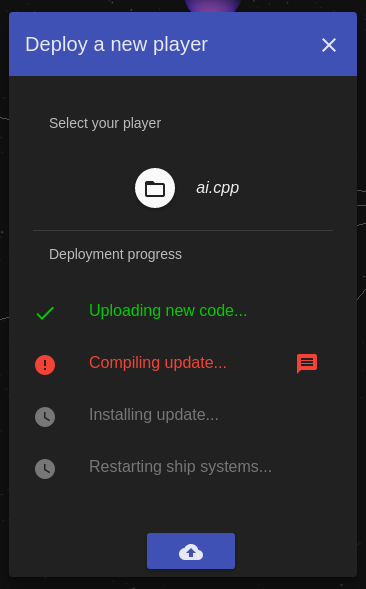
\includegraphics{images/deploy_error.png}
}
}
\caption{Player deployment with a compilation error}
\label{deploy_error}
\end{figure}
\end{minipage}
\begin{minipage}{.5\textwidth}
\begin{figure}[H]
\makebox[\textwidth]{
\noindent\resizebox{!}{100pt}{
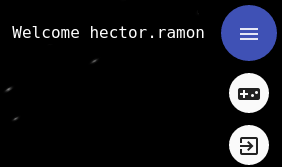
\includegraphics{images/player_menu.png}
}
}
\caption{Player menu}
\label{player_menu}
\end{figure}
\end{minipage}
\end{figure}
\section{Summary}
This chapter detailed the implementation of the \texttt{AI} hot-swapping feature, which needed an
authentication system first. Summarizing, the most important implemented components are:
\begin{enumerate}
\item
The \texttt{PLAYER\_EXISTS} and \texttt{DEPLOY\_PLAYER} request handlers in the engine app-server
\item
The \texttt{/auth} and \texttt{/player} endpoint in the \texttt{API}
\item
The login form, player menu, and deployment form in the viewer.
\end{enumerate}
\chapter{The control panel}
\label{control_panel}
Given that an authentication system was available, it was then possible to create a control panel
to allow administrators control the current match.
\section{Recognizing administrators}
At this point, the platform did not know anything about administrators, only players.

An administrator is a user that has privilege to control the current match. Given that administrators were not used
in the game logic, it did not make sense to add them in the engine. Hence, the concept was added in the \texttt{API}, as a way
to control access to some engine operations.

The \texttt{API} was changed to read a file when booting up that contained a list of user identifiers that should be considered
administrators. Then, the \texttt{/auth} endpoint was changed to allow administrators login even if they did not have an associated
player in the engine.
\section{Assuming control}
New types of request handlers were added to the engine app-server that allowed to pause and play the match: \texttt{PLAY\_MATCH} and
\texttt{PAUSE\_MATCH}, respectively.

These new handlers were exposed through the \texttt{API} in the new endpoints: \texttt{/control/play} and \texttt{/control/stop}. Obviously,
these endpoints checked that the authenticated user requesting the action was an administrator. If not, a \texttt{403 Forbidden}
error was returned.

Finally, a simple control panel was added in the viewer to allow administrators control the match.
\chapter{The first game world}
\label{first_game_world}
Before going any further, it was convenient to make a quick review of the current state of the platform. At this point,
the platform was able to:
\begin{enumerate}
\item
Notify game events in real-time
\item
Replay the past of the current match
\item
Hotswap \texttt{AIs} during a match
\end{enumerate}
These features alone, fullfilled 2 of the 6 secondary objectives detailed in \autoref{secondary_objectives},
specifically:
\begin{enumerate}
\item
Allow hot-swapping of \texttt{AIs}
\item
Implement a real-time webviewer
\end{enumerate}
Therefore, there were still four secondary objectives to fullfill. However, one of these objectives talked about
stability and scalability, features that could only be validated at the end of the project (see \autoref{validation}).

For this reason, it was decided that the next implemented features aimed to fullfill the objectives:
\begin{enumerate}
\item
Develop an abstract game engine
\item
Create a game example
\end{enumerate}
These two objectives could be fullfilled both at the same time by creating a game example without adding any game-specific
code in the engine. To achieve that, a set of abstract classes were created in the engine to build game logic on top of them:
\begin{description}
\item[\texttt{Game}]
Used to configure general aspects of the game and as a factory of game \texttt{World}s and \texttt{Action}s.
\item[\texttt{World}]
Used to implement game update logic and world serialization.
\item[\texttt{AI}]
Used to build the interface that players will have available when implementing \texttt{AIs}.
\item[\texttt{Action}]
Used to implement action logic and serialization.
\end{description}
These classes allowed game developers to build \texttt{MMPGs} while extending the engine code, not changing it.
\section{Choosing a game: Space Wars}
First, it was necessary to choose the game to implement. The best candidates were games with simple rules, but that
also seemed easy to extend. Hence, development could start with the implementation of the original game rules while
new ideas to increase the game size and make it massive could be added later.

At the end, it was chosen to implement a game inspired by Galcon \cite{galcon}, which also inspired
Planet Wars \cite{planet_wars}. Planet Wars was a game used in the \texttt{AI} programming challenge
(see \autoref{state_of_the_art}) sponsored by Google during 2010. The game rules are simple:
\begin{enumerate}
\item
The game world consists in a system with a determined number of planets.
\item
Every player owns one planet before the match starts.
\item
During the match, every owned planet generates space ships in a rate that is proportional to the radius of the planet.
\item
Ships can be sent from planet to planet.
\item
A player can conquer other planets by sending a greater number of ships than the planet holds.
\item
The objective of the match is to destroy other players and/or conquer the major number of planets.
\end{enumerate}
These rules make an interesting strategic game that is quite convenient for a programming game.

The code of the game example can be found in the \texttt{space-wars-game} GitHub organization: \url{https://github.com/space-wars-game}.
\section{Generating a planetary system}
The first step to implement the game rules was to generate a game world: a planetary system.

In order to make every match different, it was decided to generate the game world procedurally using a pseudo-random
generator\footnote{Mersenne Twister \cite{mersenne_twister}}.

A simplified model of a realistic planetary system was taken. A planetary system in the game had one sun and a
determined number of planets. A planet was assumed to move describing an ellipse with the sun as its center.
Thus, assuming the position of the sun was $(0, 0)$, then the coordinates $x$ and $y$ of the planet were

$$x = a \: cos \theta$$
$$y = b \: sin \theta$$

where $a$ and $b$ were the major and minor axes of the ellipse, respectively, and $\theta$ was the eccentric anomaly.

Algorithm \autoref{system_generation} shows the algorithm used to generate planetary systems procedurally in the game.
Basically, the algorithm generated planets outwards from the sun, while ensuring their orbits did not collide,
and positioned them on a random point of its orbit.
\begin{algorithm}
\caption{Procedural generation of planetary systems}
\label{system_generation}
\begin{algorithmic}
\STATE{$sun \gets Sun(in\_range(\text{Sun::MIN\_RADIUS}, \text{Sun::MAX\_RADIUS}))$}
\STATE{$num\_planets \gets in\_range(\text{System::MIN\_SIZE}, \text{System::MAX\_SIZE})$}
\STATE{$planets \gets \text{list of } num\_planets \text{ planets}$}
\STATE{$previous \gets sun$}
\FOR{$p \text{ in } planets$}
\STATE{$p_{radius} \gets in\_range(\text{Planet::MIN\_RADIUS}, \text{Planet::MAX\_RADIUS})$}
\STATE{$dist_x \gets in\_range(\text{Planet::MIN\_DIST\_X}, \text{Planet::MAX\_DIST\_X})$}
\STATE{$dist_y \gets in\_range(\text{Planet::MIN\_DIST\_Y}, \text{Planet::MAX\_DIST\_Y})$}
\STATE{$p_a \gets previous_a + dist_x + p_{radius} + previous_{radius}$}
\STATE{$p_b \gets previous_b + dist_y + p_{radius} + previous_{radius}$}
\STATE{$p_\theta \gets in\_range(0, 2\pi)$}
\STATE{$previous \gets p$}
\ENDFOR
\end{algorithmic}
\end{algorithm}
\clearpage
\section{Connecting planets}
At this point, it was possible to generate a planetary system as the game world. However, it was decided that a planet
could not send ships to any other planet, but only to planets that were connected to it, unlike the original Galcon \cite{galcon}.
As a consequence, the game became more interesting, encouraging players to learn path-finding techniques.

Hence, it was necessary to also generate a connected graph of planets. Algorithm \autoref{connection_generation} shows
the algorithm used to generate the planetary connections procedurally.
\begin{algorithm}[H]
\caption{Procedural generation of planetary connections}
\label{connection_generation}
\begin{algorithmic}
\REQUIRE{$p \text{ is a list of planets}$}
\STATE{$relay \gets p[in\_range(0, p_{length})]$}
\STATE{$connected \gets \text{queue of planets}$}
\STATE{$disconnected \gets p - relay$}
\STATE{$\text{push } relay \text{ to } connected$}
\WHILE{$disconnected \text{ is not empty}$}
\STATE{$edge \gets \text{front of } connected$}
\STATE{$\text{pop front of } connected$}
\STATE{$max\_connections \gets min(\text{Planet::MAX\_CONNECTIONS}, disconnected_{length})$}
\STATE{$num\_connections \gets in\_range(\text{Planet::MIN\_CONNECTIONS}, max\_connections)$}
\FOR{$i \text{ in } (0, num\_connections)$}
\STATE{$c \gets disconnected[in\_range(0, disconnected_{length})]$}
\STATE{$\text{add } c \text{ to } edge_{connections}$}
\STATE{$\text{add } edge \text{ to } c_{connections}$}
\STATE{$disconnected \gets disconnected - c$}
\STATE{$\text{push } c \text{ to } connected$}
\ENDFOR
\ENDWHILE
\end{algorithmic}
\end{algorithm}
\section{Rendering the planetary system}
Finally, the viewer was upgraded to render the generated planetary system and its connections.

Basically, OpenGL spheres were used to draw the sun and the planets, while connections were represented
using lines. Additionally, a light was added in the center of the sun to give some depth to the scene.

\autoref{render_system} shows a planetary system rendered by the viewer.
\begin{figure}[H]
\noindent\resizebox{\textwidth}{!}{
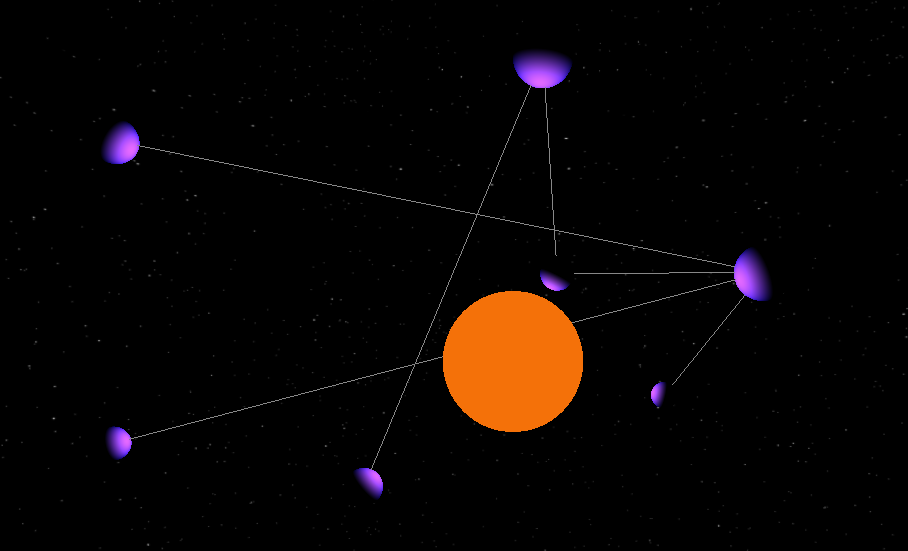
\includegraphics{images/planets.png}
}
\caption{Planetary system rendered by the viewer}
\label{render_system}
\end{figure}
\section{Summary}
This chapter detailed how the implementation of the game example started:
\begin{enumerate}
\item
It was chosen to create a game inspired by Galcon \cite{galcon}.
\item
A simple algorithm was implemented to procedurally generate the game world.
\item
The viewer was upgraded to render the generated game world.
\end{enumerate}
\chapter{Fleets and planets}
\label{fleets_planets}
At this point, a planetary system was being generated as the game world. Thus, it was possible to start developing 
the main game mechanics: ship generation and fleet movement.
\section{Generating ships in conquered planets}
The ship generation mechanic states that conquered planets generate ships at a rate proportional to the
radius of the planet. Hence, the bigger the planet, the more ships it will generate during a specific timeframe.

The nature of this mechanic is periodical: conquered planets need to be updated quite frequently. Games can easily
implement this type of mechanics because their entire logic is executed in a game loop.

A game loop is the central code of a game. It is a loop that is executed constantly to update the state of
the game accordingly. A good game loop computes the time between iterations and has a fixed timestep, which ensures
that the update logic always advances the state of the game in the same amount.

Algorithm \autoref{game_loop} shows an example of a game loop with a fixed timestep. This type of game loop
avoids differences in game speed between different hardware, while it also avoids passing a big timestep to the
update logic, which could break game calculations\footnote{like collision detection, movement, etc.}.

At the end, the engine was upgraded to support a game loop with a fixed timestep. The timestep could be configured
by extending the \texttt{Game} class described in \autoref{first_game_world}. Then, the corresponding update logic was
implemented in the game logic to generate ships in conquered planets as described by the game mechanic.
\begin{algorithm}
\caption{Game loop with a fixed timestep}
\label{game_loop}
\begin{algorithmic}
\STATE{$accum \gets 0$}
\STATE{$time_{current} \gets current\_time()$}
\WHILE{$\text{not } quit$}
\STATE{$time_{new} \gets current\_time()$}
\STATE{$time_{frame} \gets time_{new} - time_{current}$}
\STATE{$time_{current} \gets time_{new}$}
\STATE{$accum \gets accum + time_{frame}$}
\WHILE{$accum \geq timestep$}
\STATE{$update\_state(timestep)$}
\STATE{$accum \gets accum - timestep$}
\ENDWHILE
\ENDWHILE
\end{algorithmic}
\end{algorithm}
\section{Moving fleets between planets}
The fleet movement mechanic describes how players can send ships from a planet to another.

Basically, it was implemented assuming that a fleet trip is defined by:
\begin{itemize}
\item
Planet origin
\item
Planet destination
\item
Fleet owner
\item
Number of ships
\item
Travel time
\end{itemize}
The travel time was proportional to the euclidean distance between the planet origin $o$ and the planet destination $d$,
assuming that every fleet moved at the same velocity $v$:

$$t_{time} = \frac{\sqrt{(d_x - o_x)^2 + (d_y - o_y)^2}}{v}$$

The velocity value was constant in the game, but it could be easily changed to experiment with different values.

Then, in the update logic, every on-going fleet trip was updated properly, applying changes to the destination planets
when a trip finished. Algorithm \autoref{trip_algorithm} and \autoref{planet_algorithm} give a basic idea of how the trip and planet
update logics were implemented, respectively.
\begin{algorithm}[H]
\caption{Fleet trip update logic}
\label{trip_algorithm}
\begin{algorithmic}
\FOR{$t \text{ in } current\_trips$}
\STATE{$t_{time} \gets t_{time} - timestep$}
\IF{$t_{time} \leq 0$}
\STATE{$update\_planet(t_{destination}, t)$}
\STATE{$current\_trips \gets current\_trips - t$}
\ENDIF
\ENDFOR
\end{algorithmic}
\end{algorithm}
\begin{algorithm}[H]
\caption{Planet update logic}
\label{planet_algorithm}
\begin{algorithmic}
\REQUIRE{$p \text{ is a planet}$}
\REQUIRE{$t \text{ is a fleet trip}$}
\IF{$\text{not } p_{owner}$}
\STATE{$p_{owner} \gets t_{owner}$}
\ENDIF
\IF{$p_{owner} = t_{owner}$}
\STATE{$p_{ships} \gets p_{ships} + t_{ships}$}
\ELSE
\IF{$p_{ships} \geq t_{ships}$}
\STATE{$p_{ships} \gets p_{ships} - t_{ships}$}
\ELSE
\STATE{$p_{owner} \gets t_{owner}$}
\STATE{$p_{ships} \gets t_{ships} - p_{ships}$}
\ENDIF
\ENDIF
\end{algorithmic}
\end{algorithm}
\section{Rendering fleets and planet information}
Finally, the viewer was upgraded to render fleets moving between planets. Octahedrons were used to represent
fleets, scaling them proportionally to the number of ships. Fleets movement was animated using the planet origin,
planet destination and travel time.

Additionally, the viewer was modified to show planet information: number of ships and owner. These elements were
projected on top of the \texttt{3D} viewer using \texttt{HTML} elements.

A simple \texttt{AI} was implemented and two players were confronted with each other to test these mechanics and the viewer together.
\autoref{player_ai} shows the code of the developed \texttt{AI}, while \autoref{viewer_fleets} shows an example of a match
played by two players using this \texttt{AI}.
\begin{figure}[H]
\inputminted[linenos,fontsize=\small,frame=lines,framesep=2mm]{c++}{code/ai.cpp}
\caption{A simple \texttt{AI} that tries to conquer all the planets}
\label{player_ai}
\end{figure}
\begin{figure}[H]
\noindent\resizebox{\textwidth}{!}{
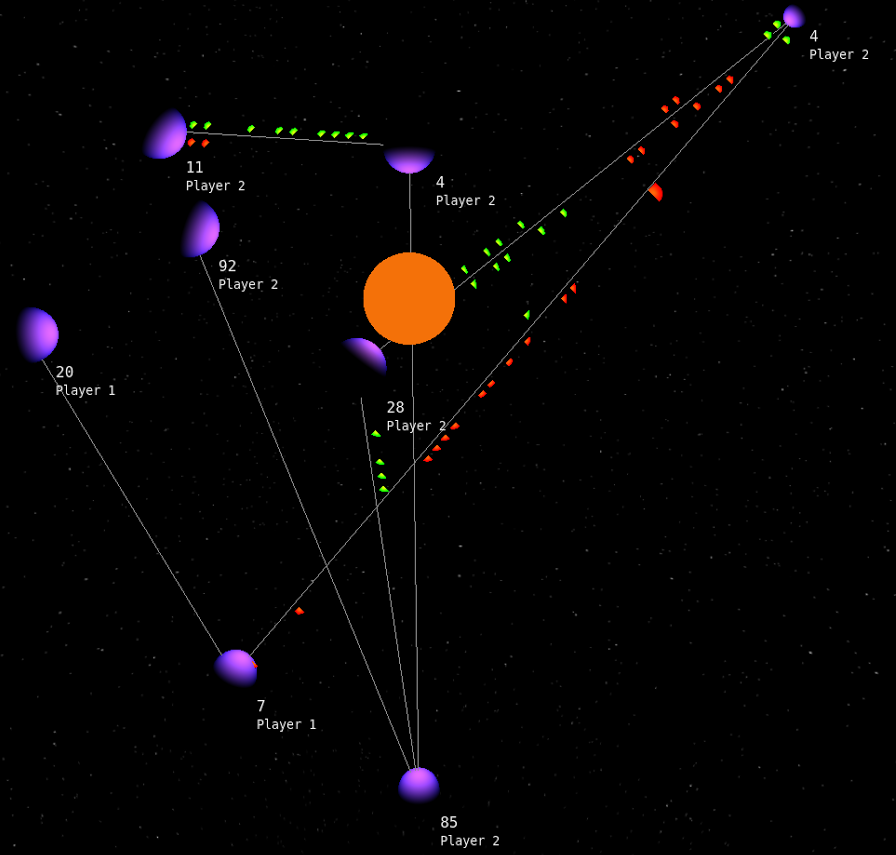
\includegraphics{images/viewer_fleets.png}
}
\caption{The viewer showing fleets and planet information}
\label{viewer_fleets}
\end{figure}
\section{Summary}
In this chapter, the basic mechanics of the game example were developed. The implementation process consisted in:
\begin{enumerate}
\item
Adding game loop support to the engine
\item
Implementing the ship generation logic
\item
Implementing the fleet movement logic
\item
Upgrading the viewer to show fleets and planet information
\end{enumerate}
\chapter{A whole galaxy}
\label{whole_galaxy}
At this point, the integration server was running a game similar to Galcon: a small number of players could
compete to win control over the generated planetary system. However, it was necessary to increase the game size
in order to add support for a high amount of players.
\section{Generating multiple planetary systems}
At this moment, the game world was a planetary system. Therefore, the logical step to increase the game size
was to think about a galaxy.

The game size was increased by generating a number of planetary systems proportional to the amount
of players of the match. Different systems were connected using an algorithm similar to the one used to
connect planets (described in \autoref{fleets_planets}). A new type of celestial body was added to each system that
allowed ships to travel to its connected systems: the relay.

In order to simplify the galaxy generation, it was decided that the system position would not affect travel time between
systems. Specifically, travelling from one relay to another was instantaneous. This way, a galaxy could be simplified
to an ordered set of systems, with no need to positionate the systems correctly inside the game logic.
\section{Separating world structure from dynamic data}
Once the new world generation was ready, a new prototype was deployed to the integration server. This prototype
generated 300 systems as the game world.

After deploying the prototype, the CPU usage in the server increased from 1-2\% to 20\%. While an increase
in the CPU usage was expected, it was not expected to be that high. Hence, an analysis was performed to detect
any possible bottlenecks.

The main detected symptom was that the \texttt{API} was notifying 200 kbits of events per second, when the bandwidth needed was 10-12 kbps
before deploying. The events that changed after the deployment were the snapshots (see \autoref{log_system}).
The game world increased its size by 300 times, thus the snapshots were approximately 300 times bigger. These snapshots
were also sent to players quite often to keep their copies of game worlds updated.

Given that the snapshot generation turned expensive, an optimization was needed. Most of the generated game world was static,
it did not change: a system stayed with the same structure the entire match. The only data that could potentially change
was the number of ships and the owner of every planet. Thus, there was no reason to constantly generate snapshots where most of
their data was static. Instead, static data and dynamic data could be separated.

Therefore, the optimization consisted in generating a world structure snapshot only once, and notify it to players and
viewers only once. Then, snapshots containing dynamic data were generated and notified periodically, as before.

The optimization reduced the CPU usage from 20\% to 3\% consistently and the bandwidth from 200kbps to 20kbps.
\autoref{cpu_galaxy} shows the CPU usage drop after the optimization was deployed.
\begin{figure}[H]
\noindent\resizebox{\textwidth}{!}{
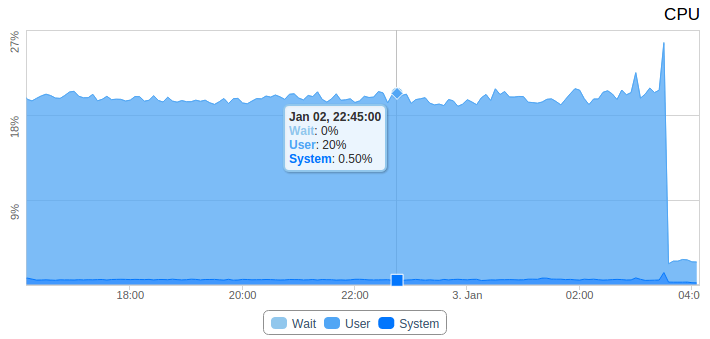
\includegraphics{images/cpu_galaxy.png}
}
\caption{CPU usage drop after separating world structure from dynamic data}
\label{cpu_galaxy}
\end{figure}
\section{Rendering a galaxy}
After the optimization, the game logic was mostly finished. Space Wars was able to scale its size with the number of players
efficiently. Hence, the last task left to finish the game was to upgrade the game viewer so it could show the generated galaxy.

The idea was to show a galaxy map. Basically, the galaxy map would show a general view of all the game world. In other words,
it would show every system in a clear way. However, as it was said before, the galaxy is just an ordered set of systems.
A system did not have a particular position in the game logic. As a consequence, the viewer had the responsibility to turn this
ordered set into a galaxy.

Now, galaxies come in different shapes \cite{galaxy_shapes}, but the most familiar of them is the spiral shape. Our galaxy,
the Milky Way has an spiral shape, as shown by \autoref{milky_way}.
\begin{figure}[H]
\begin{center}
\noindent\resizebox{.9\textwidth}{!}{
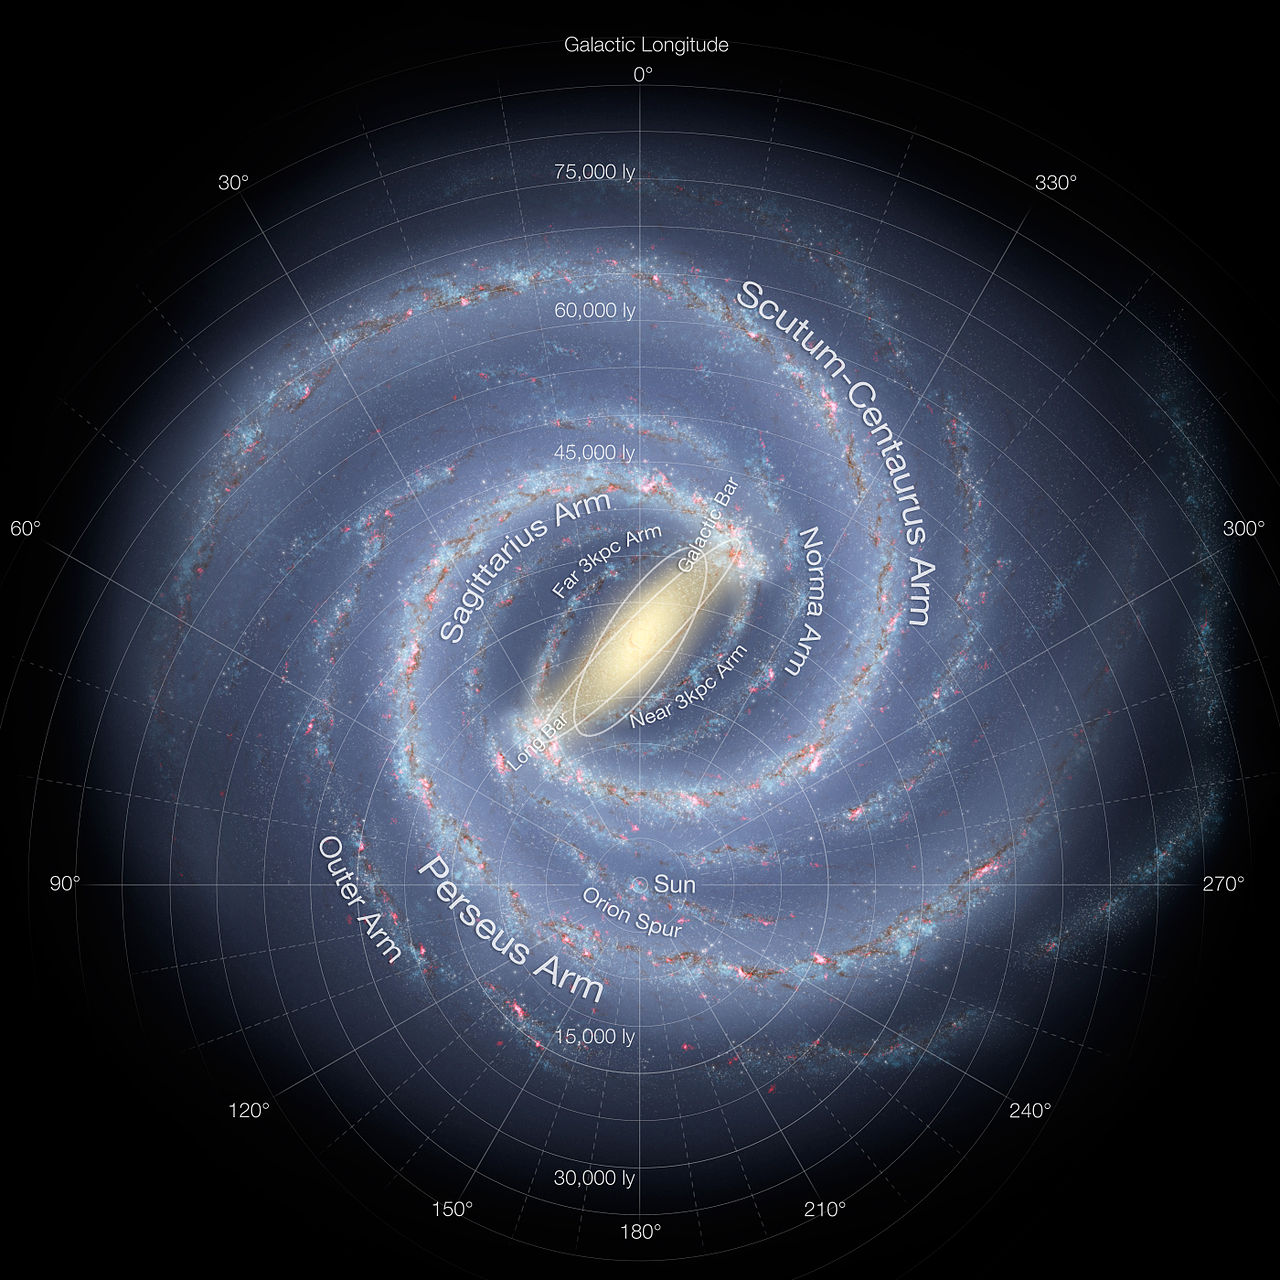
\includegraphics{images/milky_way.jpg}
}
\end{center}
\caption{Artist's conception of the spiral structure of the Milky Way \cite{milky_way_concept}}
\label{milky_way}
\end{figure}
Hence, in order to simulate an spiral galaxy, it was necessary to study the spiral equations \cite{spiral_equations} first.

Basically, the coordinates of the points in a spiral are defined by

$$x(t) = at \: cos(t)$$
$$y(t) = at \: sin(t)$$

where $t$ is an angle and $a$ is a constant that controls the spiral density.

However, spiral galaxies can have multiple arms. This means that they can be formed by multiple spirals with different rotations.
A spiral can be easily rotated by an angle $\theta$:

$$x(t) = at \: cos(t + \theta)$$
$$y(t) = at \: sin(t + \theta)$$

Using these last equations, it was relatively easy to build a simple algorithm that assigned a position $(x, y)$ to every
planetary system of the game world, while generating a galaxy with a number of arms proportional to the number of systems.
Algorithm \autoref{spiral_algorithm} shows the algorithm used to generate the galaxy map.
\begin{algorithm}[H]
\caption{Galaxy map generation}
\label{spiral_algorithm}
\begin{algorithmic}
\REQUIRE{$systems \text{ is a list of systems}$}
\REQUIRE{$\alpha \text{ is the initial angle}$}
\REQUIRE{$arm_{systems} \text{ is the amount of systems per arm}$}
\STATE{$\theta \gets 0$}
\STATE{$t \gets \alpha$}
\STATE{$\theta_{inc} \gets 2 \pi \frac{arm_{systems}}{systems_{length}}$}
\STATE{$t_{inc} \gets \frac{2 \pi}{arm_{systems}}$}
\FOR{$s \text{ in } systems$}
\STATE{$s_x \gets a \cdot t \cdot cos(t + \theta)$}
\STATE{$s_y \gets a \cdot t \cdot sin(t + \theta)$}
\STATE{$t \gets t + t_{inc}$}
\IF{$t \geq 2 \pi + \alpha$}
\STATE{$t \gets \alpha$}
\STATE{$\theta \gets \theta + \theta_{inc}$}
\ENDIF
\ENDFOR
\end{algorithmic}
\end{algorithm}
Additionally, an ideal way to represent players uniquely was needed. Given that the number
of players could be really high, using colors would have been a bad idea, as some players would share shades of the same
color. Hence, \texttt{GitHub}-based \texttt{Identicons} \cite{identicons} were used to identify different players. The \texttt{Identicons} are
generated using player identifiers, thus players can keep the same \texttt{Identicon} in different matches.

\autoref{galaxy_map} shows an example of a galaxy rendered by the game viewer.
\begin{figure}[H]
\begin{center}
\noindent\resizebox{.75\textwidth}{!}{

\includegraphics{images/galaxy_map.png}
}
\end{center}
\caption{The Space Wars galaxy map showing an spiral galaxy with 6 arms and 300 systems}
\label{galaxy_map}
\end{figure}
\section{Summary}
This chapter detailed how Space Wars was made scalable with the number of players. Basically, the implementation
process consisted in:
\begin{enumerate}
\item
Generating multiple planetary systems
\item
Separating world structure from dynamic data
\item
Rendering a spiral galaxy using \texttt{Identicons}
\end{enumerate}
Once this was achieved, the first \texttt{MMPG} was finished.
\part{Evaluation}
\chapter{Validation}
\label{validation}
This chapter studies whether the project's secondary objectives described in \autoref{specification}
have been fullfiled after the implementation process. Then, after that study, it ponders whether
the solution obtained fullfills the main objective.
\section{Secondary objectives}
\subsection{Develop an abstract game engine}
During the entire implementation process, one of the main concerns has been to avoid adding any game-specific code
in the engine component.

Moreover, the engine architecture is entirely decoupled from any game built on
top of it.

Furthermore, the engine provides an abstraction that games can override to customize certain aspects:
like world generation, game-loop timestep, etc.

Hence, the objective has been achieved.
\subsection{Allow hot-swapping of AIs}
This \texttt{AI} hot-swapping feature was implemented in \autoref{deployment_ai}. Also, it has been tested constantly
thanks to the implementation methodology described in \autoref{methodology}. Thus, the objective has been achieved.
\subsection{Implement a real-time webviewer}
The engine was able to notify game events in real-time since the first prototype implemented in
\autoref{first_prototype}. Therefore, the objective has been achieved.
\subsection{Create a control panel}
The control panel was a feature implemented in \autoref{control_panel}. Hence, the objective has been achieved.

However, it might be too simplistic, as it only allows to play and pause the match.
Hence, more features will probably be needed before using it in a production environment, like
monitoring players in real-time, banning players, etc. These features should be easy to implement by
extending the engine, the \texttt{API} and the client.
\subsection{Create a game example}
Space Wars, the game example, was implemented during \autoref{first_game_world}, \autoref{fleets_planets},
and \autoref{whole_galaxy}. Therefore, the objective has been achieved.

However, the game might need some tweaking and balancing before using it in the EDA subject. Private tournaments could
be organised to test it properly.
\subsection{Make the infrastructure scalable and stable}
First, the platform was designed with scalability in mind:
\begin{enumerate}
\item
The engine and the \texttt{API} can work from different machines.
\item
Multiple engine workers can be used to distribute \texttt{AI} calculations in different machines.
\item
Viewers can be statically served by a simple service like \texttt{Apache} \cite{apache} or \texttt{nginx} \cite{nginx}.
\end{enumerate}

On the other hand, stability has ben assessed through continuous integration described in the implementation
methodology in \autoref{methodology}. The platform has been working 24/7 since the first prototype was deployed, without
a single crash and without any anomaly.

\autoref{mmpg_cpu} and \autoref{mmpg_io} show the CPU usage and disk IO in a period of 30 days in
the integration server, respectively. An increase in CPU usage and disk IO
can be observed when a whole galaxy was generated but it was fixed later, as it is described in \autoref{whole_galaxy}.

For these reasons, the objective has been achieved.
\begin{figure}[H]
\noindent\resizebox{\textwidth}{!}{
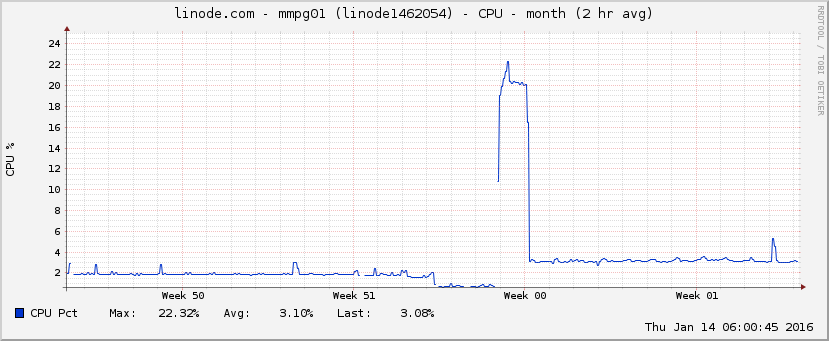
\includegraphics{images/mmpg_cpu.png}
}
\caption{CPU usage of the platform in a 30 day period}
\label{mmpg_cpu}
\end{figure}
\begin{figure}[H]
\noindent\resizebox{\textwidth}{!}{
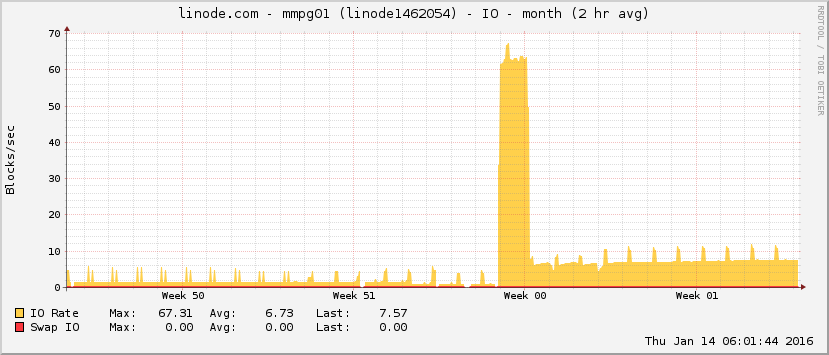
\includegraphics{images/mmpg_io.png}
}
\caption{Disk IO of the platform in a 30 day period}
\label{mmpg_io}
\end{figure}
\section{Main objective}
The main objective of the project is:
\begin{quote}
\emph{Develop a set of components that ease the creation and the usage of massive multiplayer programming games.}
\end{quote}
The abstract game engine allows game developers to build the logic of an \texttt{MMPG}, while the client library allows them
to build the viewer of an \texttt{MMPG}. Moreover, the engine supports \texttt{AI} hot-swapping natively, allowing players to change their
programs. Also, a game example has been developed to show that the platform works: Space Wars.

However, real documentation about how to use the platform is lacking. While the game example could be used by developers to
learn about the platform, it is not easy to learn from code. Thus, the main objective might not be
achieved completely until some documentation is written.

Once the lack of documentation is solved, it will be possible to say that the platform sets the foundations for a
new type of programming games: the \texttt{MMPGs}, while providing a useful set of components to create them and use them. Thus,
the main objective will be achieved.
\chapter{Time management}
This chapter details the final time arrengement of the project and compares it with the original time planning.
It shows the final duration for every task in a timetable and a timeline of how tasks were performed, while it
also studies the dedication given to the project.
\section{Time table}
\begin{figure}[H]
\begin{center}
\begin{tabular}{l S S}
\textbf{Task} & \textbf{Planned duration (h)} & \textbf{Final duration (h)}\\
\hline
Project management course & 75 & 70\\
Analysis and design & 10 & 20\\
Engine & 70 & 100\\
API & 50 & 30\\
Client & 30 & 30\\
Control panel & 35 & 15\\
Game example & 100 & 100\\
Testing and polishing & 40 & 40\\
Project memory & 40 & 50\\
Oral presentation & 10 & 10\\
\hline
\hline
\textbf{Total} & 460 & 465\\
\end{tabular}
\end{center}
\caption{Time table}
\label{time_table}
\end{figure}
\autoref{time_table} shows the final duration for every task of the project.

The main differences with the original time planning are:
\begin{itemize}
\item
The engine took more time to implement than it was expected. Mainly because of the optimization
  performed in \autoref{whole_galaxy}.
\item
The \texttt{API} was implemented faster than planned. The Go programming language resulted really easy to
  learn and use, while the native libraries made the entire implementation process really productive.
\item
The control panel was integrated in the viewer, not in the Jutge.org platform. As a result,
  it took less time to implement it, as learning the Jutge.org environment was not necessary.
\item
The project memory took more time to write than expected.
\end{itemize}
\section{Timeline}
\begin{figure}[H]
\makebox[\textwidth]{
\noindent\resizebox{\textwidth}{!}{
\begin{ganttchart}[hgrid, vgrid]{1}{25}
\gantttitle{2015}{20}
\gantttitle{2016}{5}
\\
\gantttitle{September}{5}
\gantttitle{October}{5}
\gantttitle{November}{5}
\gantttitle{December}{5}
\gantttitle{January}{5}
\\
\ganttbar{Project management}{3}{11}
\\
\ganttbar{Analysis and design}{6}{7}
\\
\ganttbar{Engine}{11}{20}
\\
\ganttbar{API}{11}{20}
\\
\ganttbar{Client}{11}{20}
\\
\ganttbar{Space Wars - logic}{16}{21}
\\
\ganttbar{Space Wars - viewer}{16}{21}
\\
\ganttbar{Testing and polishing}{13}{22}
\\
\ganttbar{Project memory}{16}{23}
\\
\ganttbar{Oral presentation}{24}{24}
\ganttlink{elem1}{elem2}
\ganttlink{elem1}{elem3}
\ganttlink{elem1}{elem4}
\ganttlink{elem8}{elem9}
\end{ganttchart}
}
}
\caption{Final timeline}
\label{final_timeline}
\end{figure}
\autoref{final_timeline} shows the final timeline for every task of the project.

The main difference can be observed in the testing and polishing task. As the implementation methodology
used continuous integration (\autoref{methodology}), the testing and polishing of the platform has been
constant since the first prototype (\autoref{first_prototype}). Also, the different components have been developed
at the same time, in order to have a fully-functional prototype after each iteration.
\section{Dedication}
\autoref{dedication} shows the relative amount of contributions per day to this project.
\begin{figure}[H]
\makebox[\textwidth]{
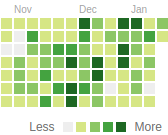
\includegraphics[scale=0.6]{images/dedication.png}
}
\caption{GitHub contributions to the \texttt{MMPG} project \url{https://github.com/hecrj}}
\label{dedication}
\end{figure}
At least one contribution was made every day since the 2nd of November of 2015, with only two days being the exception.
As a consequence, the project has been in constant progress; new features were added to the fully-functional
prototype and were reported to the project advisor on a weekly basis.

Contribution peaks (\emph{greenest squares}) happened when some important feature or optimization was implemented, which
increased the dedication to the project during a specific timeframe.

It should be noted that \autoref{dedication} does not give any type of feedback about the testing tasks performed
in the platform during its implementation.

Overall, the amount of work has been distributed properly and the project has been developed at a steady pace.
\chapter{Economic cost}
\section{Hardware resources}
The project used the hardware resources specified in \fullref{budget}. However, a Linode 1GB was needed during 3 months.
\begin{table}[H]
\centering
\begin{tabular}{l S}
\textbf{Hardware} & \textbf{Cost (\EURtm)}\\
\hline
Hardware budget & 60.13\\
Linode 1GB & 27.47\\
\multicolumn{1}{l }{\textbf{Total}}
 & 87.60
\end{tabular}
\caption{Hardware cost}
\label{Hardware cost}
\end{table}
\section{Software resources}
As stated in the original planning, all the software needed to develop the project can be used for free.
  \autoref{Additional software} shows additional software that was used but it was not listed in the original planning.
\begin{table}[H]
\centering
\begin{tabular}{l l}
\textbf{Software} & \textbf{License}\\
\hline
\texttt{Three.js} & \url{https://github.com/mrdoob/three.js/blob/master/LICENSE}\\
\texttt{Identicon}.js & \url{https://github.com/hecrj/identicon.js/blob/master/LICENSE}\\
\end{tabular}
\caption{Additional software}
\label{Additional software}
\end{table}
\section{Human resources}
\autoref{Human resources cost} shows the final cost of the human resources according
to the final task durations detailed in \autoref{time_table} and the salary per role in \autoref{Salary per role}.
\begin{table}[H]
\centering
\begin{tabular}{l l S S}
\textbf{Role} & \textbf{Task} & \textbf{Time (h)} & \textbf{Cost (\EURtm)}\\
\hline
\multirow{3}{*}{Project manager}
 & Project management course & 70 & 2450.00\\
 & Project memory & 50 & 1750.00\\
 & Oral presentation & 10 & 350.00\\
\hline
\multirow{1}{*}{Software engineer}
 & Analysis and design & 20 & 800.00\\
\hline
\multirow{6}{*}{Software developer}
 & Engine & 100 & 3000.00\\
 & API & 30 & 900.00\\
 & Client & 30 & 900.00\\
 & Control panel & 15 & 450.00\\
 & Game example & 100 & 3000.00\\
 & Testing and polishing & 40 & 1200.00\\
\hline
\hline
\multicolumn{2}{l }{\textbf{Total}}
 & 465.00 & 14525.00
\end{tabular}
\caption{Human resources cost}
\label{Human resources cost}
\end{table}
\section{Other resources}
\subsection{Electricity}
\autoref{Electricity cost} shows the electricity cost of the project.
\begin{table}[H]
\centering
\begin{tabular}{l S S S}
\textbf{Hardware} & \textbf{Consumption (W)} & \textbf{Time of usage (h)} & \textbf{Cost (\EURtm)}\\
\hline
Desktop computer & 400 & 440 & 25.94\\
Laptop & 100 & 5 & 0.07\\
Monitor Acer XB270HU & 30 & 440 & 1.95\\
\hline
\hline
\multicolumn{3}{l }{\textbf{Total}}
 & 27.95
\end{tabular}
\caption{Electricity cost}
\label{Electricity cost}
\end{table}
\subsection{Internet connection}
The project was developed using the internet connection described in \autoref{budget}. The internet connection was used
approximately during the 30\% of the total project's duration, as expected.
Thus, the final cost of the internet connection was 465h $\cdot$ 0.05\EURtm/h $\cdot$ 0.3 $=$ 7.36\EURtm.
\clearpage
\section{Total}
\autoref{Total cost} shows the total cost of the project compared to the budget of the planning stage.
\begin{table}[H]
\centering
\begin{tabular}{l S S}
\textbf{Resource} & \textbf{Budget (\EURtm)} & \textbf{Total cost (\EURtm)}\\
\hline
Hardware & 60.13 & 87.60\\
Software & 0.00 & 0.00\\
Human & 14525.00 & 14800.00\\
Electricity & 26.08 & 27.95\\
Internet & 7.28 & 7.36\\
\hline
Contingency (10\%) & 1461.85 & 0.00\\
\hline
\hline
\multicolumn{1}{l }{\textbf{Total}}
 & 16080.34 & 14922.91
\end{tabular}
\caption{Total cost}
\label{Total cost}
\end{table}
\chapter{Sustainability}
This chapter contains a basic sustainability report of the project based on the method described by
Christian Felber in `The economy of the common good' \cite{sustainability_report}.
\section{Economic analysis}
The economical analysis was complete and thorough, all costs are assessed and reasonable.
Resources were used efficiently, more time was spenth in the most important tasks. Moreover, the best technologies
were chosen to produce the best results in the least amount of time possible. A contingency budget was added
to take care of any unexpected problems.

However, the project is not aimed to be profitable, so there will be no direct economic benefit from it.
\section{Social impact analysis}
The project is directed to computer science students and teachers, and game progammers. The project
will be used by students to learn different programming techniques, by teachers to evaluate these students, and
by game programmers to create new content.

Moreover, it will be used in the EDA subject at the FIB. The project will make the learning process more fun, it will also
reduce the amount of work for teachers, and it will make game programmers able to create entertaining games easily.

However, the project will not affect the mainstream consumer directly. It will only be relevant inside a specific
community in computer science and education.
\section{Environmental impact analysis}
The project used 177kWh of electricity, which is approximately 174kg of CO\textsuperscript{2} \cite{co2}.
This is the amount of CO\textsuperscript{2} that a car produces by driving only 7
hours\footnote{\url{http://www.yousustain.com/footprint/howmuchco2?co2=174+kg}}. Also, any source of
information was accessed digitally over the internet.

However, the hardware used can not be fully recycled and it will, eventually, become electronic waste
with a high amount of contaminants.
\chapter{Legality}
There are no special laws that apply to this project. The entity using the platform
is liable for the information inputted in it, as it is specified in the code license.
\chapter{Conclusion}
This last chapter closes the project by summarizing the document, detailing the future of the project and
giving the author personal thoughts.
\section{Summary}
This document detailed the building process of a platform for \texttt{MMPGs}.

First, the requirement for \texttt{MMPGs} games was established. Then, it was shown that there was not
an existing solution to satisfy it. Thus, the requirement was analyzed and a solution was designed. This solution
featured a set of different components that allowed the creation of \texttt{MMPGs}.

Second, the development of the solution was planned. A time plan and a budget for the solution were shown.

Next, the implementation of the solution was detailed. Starting with a prototype and using continuous integration, the different
features that the solution needed were developed.

Finally, the implemented solution was evaluated. The solution was checked against the objectives of the project,
while also showing the time management during its implemenation and its final economic cost.
\section{The future}
The future of this project is promising. Given that the platform is released as open source, the project will be maintained
by the author and, hopefully, by the community in the future.

Some of the tasks that will be performed in the near-future are:
\begin{description}
\item[Documentation]
Different types of documentation will be written:
\begin{enumerate}
\item
A guide for developers will explain how to start developing a game with the platform with detail.
\item
A guide for contributors will help developers to contribute to the project.
\item
A guide for Space Wars will teach players how to install Space Wars and develop \texttt{AIs} locally.
\item
\texttt{README}s in every component will explain its responsibility in the platform.
\end{enumerate}
\item[Widget library]
A library containing predefined viewer widgets will be implemented. Game developers will be
  able to use this widgets to implement viewer functionalities; like a login form, or the time control, for example.
\item[Game template]
A simple game will be created. This game might be used by game developers as a starting point.
  Forking the repository of this game will give game developers a simple fully-functional game out-of-the-box.
\item[Game-logic testing suite]
The engine will get its own testing suite, so game developers will be able test the logic
  of their games effortlessly.
\end{description}
\section{Personal thoughts}
It is difficult to express my thoughts after such a long project.

When I started, I did not imagine I would have to develop so many different components at the same time. However, I really
liked the implementation methodology used in the project. Being able to deploy changes automatically and show them
to anyone was motivating. Also, it surprises me how low the time spent debugging has been. Bugs were detected
and fixed really fast.

I have learned a lot during this project. I did not know how to code in \texttt{Go} when I started. Right now, it is
another tool in my toolbox. \texttt{Three.js} was also new to me, and I've been amazed by how powerful it is. I have also learned about 
the different low-level libraries to implement inter-process communication, which I had never used for anything serious
before this project. Moreover, procedural generation was one of those topics that interested me but never tried.
I have been constantly learning and mixing my knowledge with new concepts.

I have mixed feelings with the outcome of this project. I think it is really promising, but I would have liked to
offer a more finished and better documented solution.

At the end, though, developing this project has been a really fun and rewarding experience and I am sure it will
benefit me deeply in my incoming professional career.
\bibliographystyle{plain}
\bibliography{references}
\end{document}
